% \def\year{2018}\relax
%File: formatting-instruction.tex

% AAAI mandatory header
% \documentclass[letterpaper]{article} %DO NOT CHANGE THIS
% \usepackage{aaai18}  %Required
% \usepackage{times}  %Required
% \usepackage{helvet}  %Required
% \usepackage{courier}  %Required
% \usepackage{url}  %Required
% \usepackage{graphicx}  %Required
% \frenchspacing  %Required
% \setlength{\pdfpagewidth}{8.5in}  %Required
% \setlength{\pdfpageheight}{11in}  %Required
% %PDF Info Is Required:
% \pdfinfo{
% 	/Title (A Convolutional Approach to Learning Time Series Similarity)
% 	/Author (Anonymous)}
% \setcounter{secnumdepth}{0}

% % ICLR mandatory (?) header
% \documentclass{article} % For LaTeX2e
% \usepackage{iclr2018_conference,times}
% \usepackage{hyperref}
% \usepackage{url}

%\iclrfinalcopy % Uncomment for camera-ready version, but NOT for submission.

% KDD / ACM sigconf version
\documentclass[sigconf]{acmart}
\setcopyright{rightsretained}
\acmDOI{10.475/123_4}
\acmISBN{123-4567-24-567/08/06}
\acmConference{KDD'19}{}{August 19--23, 2018, London, United Kingdom.}
\acmYear{2018}
\copyrightyear{2018}
\fancyhead{}

%-------------------------------------------------------------- Includes

\usepackage{bbm}  % who knows?

\usepackage{amsmath}          % basic math
\usepackage{amssymb} 			    % math symbols
\usepackage{amsthm}           % theorems
\usepackage{textcomp}

% \usepackage{float}            % make figures work
% \usepackage{cite}             % citations would be nice
\usepackage{url}              % better urls; magically keeping doc from breaking due to urls in refs

% \usepackage{tabu}
\usepackage{array}            % multiline table cells; somehow
\usepackage{tabularx}         % better tables
% \usepackage[table]{xcolor}    % colored table cells  % incompatible with sigconf
\usepackage{colortbl}
\newcolumntype{Y}{>{\centering\arraybackslash}X}	% centered column type for tabularx

% stuff for piecewise functions
\usepackage{mathtools}          %loads amsmath as well
\DeclarePairedDelimiter\Floor\lfloor\rfloor
\DeclarePairedDelimiter\Ceil\lceil\rceil

\DeclareMathOperator*{\argmin}{arg\,min} % argmin
\DeclareMathOperator*{\argmax}{arg\,max} % argmax

\usepackage{pbox}   % for trick to force linebreaks in table cells

\usepackage{setspace}
% \usepackage{setspace}

\usepackage{makecell}
\usepackage{hhline}

% \usepackage{booktabs} % acm recommended, and for pandas latex tables

%-------------------------------------------------------------- Algorithm setup

\usepackage{algorithm}
\usepackage[noend]{algpseudocode} % I think this removes trailing "end {if,for,while}"

% \algnewcommand{\LineComment}[1]{\State \(\triangleright\) #1} % left-aligned comments
% \algnewcommand{\SideComment}[1]{\(//\) #1}
\algnewcommand{\COMMENT}[2][.5\linewidth]{\leavevmode\hfill\makebox[#1][l]{//~#2}}
\algnewcommand{\LineComment}[1]{\State \(//\) #1}	% left-aligned comments
\algnewcommand\RETURN{\State \textbf{return} }


%-------------------------------------------------------------- Figures setup

% \usepackage[pdftex]{graphicx}
\usepackage{graphicx}
\usepackage[space]{grffile}   % allow spaces in file names
% declare the path(s) where your graphic files are
\graphicspath{{figs/}}
% and their extensions so you won't have to specify these
\DeclareGraphicsExtensions{.pdf,.jpeg,.jpg,.png}


%\textfloatsep: space between last top float or first bottom float and the text (default = 20.0pt plus 2.0pt minus 4.0pt).
%\intextsep : space left on top and bottom of an in-text float (default = 12.0pt plus 2.0pt minus 2.0pt).
\setlength{\textfloatsep}{4pt}
\setlength{\intextsep}{4pt}

% \usepackage{caption}
% \usepackage[font={small,it}]{caption}
\usepackage[font={bf}]{caption}
% \usepackage{caption}
% \setlength{\abovecaptionskip}{-2pt} % less space between captions and figures
% \setlength{\abovecaptionskip}{-5pt}	% less space between captions and figures
% \setlength{\belowcaptionskip}{-13pt}  % less space below captions
% \setlength{\belowcaptionskip}{-10pt}  % less space below captions
\setlength{\belowcaptionskip}{-4pt}	% less space below captions

\usepackage{paralist}
\setdefaultleftmargin{10pt}{10pt}{}{}{}{}

% \usepackage{changepage}
% \usepackage{tabulary}

\usepackage{outlines}
\usepackage{enumitem}
\newcommand{\ItemSpacing}{0mm}
\newcommand{\ParSpacing}{0mm}
\setenumerate[1]{itemsep={\ItemSpacing},parsep={\ParSpacing},label=\arabic*.}
% \setenumerate[2]{itemsep={\ItemSpacing},parsep={\ParSpacing},label=\arabic*.}
\setenumerate[2]{itemsep={\ItemSpacing},parsep={\ParSpacing}}

\usepackage[linewidth=1pt]{mdframed}
\mdfsetup{frametitlealignment=\center, skipabove=0, innertopmargin=1mm,
innerleftmargin=2mm, leftmargin=0mm, rightmargin=0mm}

%-------------------------------------------------------------- Miscellaneous setup

\newlength\myindent
\setlength\myindent{2em}
\newcommand\bindent{%
  \begingroup
  \setlength{\itemindent}{\myindent}
  \addtolength{\algorithmicindent}{\myindent}
}
\newcommand\eindent{\endgroup}

% remove unwanted space between paragraphs;
% it's set by the IEEE conference format, but no papers from this conference have it
% \parskip 0ex plus 0.2ex minus 0.1ex

% make vectors be bold instead of with arrows
\renewcommand{\vec}[1]{\mathbf{#1}}
% add 'mat' command to make matrices bold
\newcommand{\mat}[1]{\mathbf{#1}}

\DeclarePairedDelimiter\ceil{\lceil}{\rceil}
\DeclarePairedDelimiter\floor{\lfloor}{\rfloor}

\newtheorem{Definition}{Definition}[section]
\newtheorem{theorem}{Theorem}

% ------------------------ convenience commands
\newcommand\eps\varepsilon
\DeclareMathOperator{\infimum}{inf}
\renewcommand\inf\infty

\renewcommand{\b}[1]{\textbf{#1}}

\renewcommand{\c}{\vec{c}}
\renewcommand{\v}{\vec{v}}
\renewcommand{\r}{\vec{r}}
% \renewcommand{\t}{\vec{t}}
\newcommand{\x}{\vec{x}}
\newcommand{\xhat}{\hat{\vec{x}}}
\newcommand{\y}{\vec{y}}
\newcommand{\yhat}{\hat{\vec{y}}}
\newcommand{\z}{\vec{z}}
\newcommand{\zhat}{\hat{\vec{z}}}
\newcommand{\s}{\vec{s}}
\newcommand{\q}{\vec{q}}

\newcommand{\R}{\mathbb{R}}

\newcommand{\onehalf}{\frac{1}{2}}

\newcommand{\pie}[1]{\frac{\pi}{#1}}
% \newcommand{\pitwo}{\frac{\pi}{2}}
% \newcommand{\pifour}{\frac{\pi}{4}}

% \newcommand{\norm}[1]{\left\lVert #1 \right\rVert}
\DeclarePairedDelimiter\abs{\lvert}{\rvert}%
\DeclarePairedDelimiter\norm{\lVert}{\rVert}%

\DeclareMathOperator{\Beta}{Beta}
\DeclareMathOperator{\Normal}{\mathcal{N}}
\DeclareMathOperator{\erf}{erf}
\DeclareMathOperator{\Var}{Var}

% make *all* text 10pt
% \renewcommand{\footnotesize}{\normalsize}
% \renewcommand{\footnotesize}{\small}
% \renewcommand{\small}{\normalsize}
  % our custom macros and config

\begin{document}
% The file aaai.sty is the style file for AAAI Press
% proceedings, working notes, and technical reports.
%
\title{A Convolutional Approach to Learning Time Series Similarity}
% \author{AAAI Press\\
% Association for the Advancement of Artificial Intelligence\\
% 2275 East Bayshore Road, Suite 160\\
% Palo Alto, California 94303\\
% }
% \author{Anonymous Authors}

\author{Divya Shanmugam}
\affiliation{
  \institution{Computer Science and Artificial \\ Intelligence Laboratory}
  \institution{MIT}
}
\email{divyas@mit.edu}

\author{Davis W. Blalock}
\affiliation{
  \institution{Computer Science and Artificial \\ Intelligence Laboratory}
  \institution{MIT}
}
\email{dblalock@mit.edu}

\author{John V. Guttag}
\affiliation{
  \institution{Computer Science and Artificial \\ Intelligence Laboratory}
  \institution{MIT}
}
\email{guttag@mit.edu}

\maketitle

% ------------------------------------------------
% CCS taxonomy stuff
% ------------------------------------------------

\begin{CCSXML}
<ccs2012>
% <concept>
% <concept_id>10002950.10003648.10003671</concept_id>
% <concept_desc>Mathematics of computing~Probabilistic algorithms</concept_desc>
% <concept_significance>500</concept_significance>
% </concept>
<concept_id>10010147.10010257.10010293.10010294</concept_id>
<concept_desc>Computing methodologies~Neural networks</concept_desc>
<concept_significance>500</concept_significance>
</concept>
<concept>
<concept_id>10002950.10003648.10003688.10003693</concept_id>
<concept_desc>Mathematics of computing~Time series analysis</concept_desc>
<concept_significance>300</concept_significance>
</concept>
<concept>
<concept_id>10002950.10003648.10003688.10003696</concept_id>
<concept_desc>Mathematics of computing~Dimensionality reduction</concept_desc>
<concept_significance>300</concept_significance>
</concept>
\end{CCSXML}

\ccsdesc[500]{Computing methodologies~Neural networks}
\ccsdesc[300]{Mathematics of computing~Time series analysis}
\ccsdesc[300]{Mathematics of computing~Dimensionality reduction}

% ------------------------------------------------
\begin{abstract}
% ------------------------------------------------

Computing distances between examples is at the core of many learning algorithms for time series. Consequently, a great deal of work has gone into designing effective time series distance measures. We present Jiffy, a simple and scalable distance metric for multivariate time series. Our approach is to reframe the task as a representation learning problem---rather than design an elaborate distance function, we use a CNN to learn an embedding such that the Euclidean distance is effective. By aggressively max-pooling and downsampling, we are able to construct this embedding using a highly compact neural network. Experiments on a diverse set of multivariate time series datasets show that our approach consistently outperforms existing methods.

\end{abstract}


% ================================================================
\section{Introduction} \label{sec:intro}
% ================================================================



Measuring distances between examples is a fundamental component of many classification, clustering, segmentation and anomaly detection algorithms for time series \citep{ucrSuite,shotgunDistance,dtwClustering,dtwClusteringWarp}. Because the distance measure used can have a significant effect on the quality of the results, there has been a great deal of work developing effective time series distance measures \citep{weightedDTW,tsDiscord, bakeoff2016,dtwClustering, tsBakeoff2008}. Historically, most of these measures have been hand-crafted. However, recent work has shown that a learning approach can often perform better than traditional techniques \citep{multimodalMetric,mddtw,decade}.

% We introduce a metric learning model for time series embedding that produces a distance measure for multivariate time series comparison. 

We introduce a metric learning model for multivariate time series. Specifically, by learning to embed time series in Euclidean space, we obtain a metric that is both highly effective and simple to implement using modern machine learning libraries. Unlike many other deep metric learning approaches for time series, we use a convolutional, rather than a recurrent, neural network, to construct the embedding. This choice, in combination with aggressive maxpooling and downsampling, results in a compact, accurate network. % The learned metric outperforms state-of-the-art methods with respect to both clustering and classification of multivariate time series.

Using a convolutional neural network for metric learning \textit{per se} is not a novel idea \citep{deepLifted, facenet}; however, time series present a set of challenges not seen together in other domains, and how best to embed them is far from obvious. In particular, time series suffer from:
\begin{enumerate}
\item \textit{A lack of labeled data}. Unlike text or images, time series cannot typically be annotated post-hoc by humans. This has given rise to efforts at unsupervised labeling \citep{extract}, and is evidenced by the small size of most labeled time series datasets. Of the 85 datasets in the UCR archive \citep{ucrArchive}, for example, the largest dataset has fewer than $17000$ examples, and many have only a few hundred.
\item \textit{A lack of large corpora}. In addition to the difficulty of obtaining labels, most researchers have no means of gathering even \textit{unlabeled} time series at the same scale as images, videos, or text. Even the largest time series corpora, such as those on Physiobank \citep{physiobank}, are tiny compared to the virtually limitless text, image, and video data available on the web. 
\item \textit{Extraneous data}. There is no guarantee that the beginning and end of a time series correspond to the beginning and end of any meaningful phenomenon. I.e., examples of the class or pattern of interest may take place in only a small interval within a much longer time series. The rest of the time series may be noise or transient phenomena between meaningful events \citep{epenthesis,neverEnding}.
\item \textit{Need for high speed}. One consequence of the presence of extraneous data is that many time series algorithms compute distances using every window of data within a time series \citep{motifExact,extract,epenthesis}. A time series of length $T$ has $O(T)$ windows of a given length, so it is essential that the operations done at each window be efficient. 
\end{enumerate}

% The quality of analyses that rest on time series comparison is directly affected by the quality of the distance measure. Desirable properties of a distance measure also include simplicity, scalability, and generality across domains.

As a result of these challenges, an effective time series distance metric must exhibit the following properties:
\begin{itemize}
	\item Efficiency: Distance measurement must be fast, in terms of both training time and inference time.
	\item Simplicity: As evidenced by the continued dominance of the Dynamic Time Warping (DTW) distance \citep{dtw} in the presence of more accurate but more complicated rivals, a distance measure must be simple to understand and implement.
	\item Accuracy: Given a labeled dataset, the metric should yield a smaller distance between similarly labeled time series. This behavior should hold even for small training sets.
    %In the unsupervised case, the metric should improve the effectiveness or speed of clustering or other unsupervised learning algorithms. In both cases, it should do so even for small training sets. % clustering algorithm to observe the sources of latent variation in the time series.
\end{itemize}

Our primary contribution is a time series metric learning method, \textit{Jiffy}, that exhibits all of these properties: it is fast at both training and inference time, simple to understand and implement, and consistently outperforms existing methods across a variety of datasets.

We introduce the problem statement and the requisite definitions in Section 2. We summarize existing state-of-the-art approaches (both neural and non-neural) in Section 3 and go on to detail our own approach in Section 4. We then present our results in Section 5. The paper concludes with implications of our work and avenues for further research.

% \section{Problem Statement}
% We first define relevant terms, frame the given problem and state our assumptions.

% \begin{Definition}{\textbf{Time Series} A $D$-variable time series $\vec{t}$ of length $T$ is a sequence of real-valued vectors $t_1,\ldots,t_T, t_i \in \mathbb{R}^D$. If $D = 1$, we call $\vec{t}$ ``univariate'', and if $D > 1$, we call $\vec{t}$ ``multivariate.''}
% \end{Definition}

% \begin{Definition}{\textbf{Subsequence} A subsequence $\vec{s}$ of a time series $\t$ is a $D$-variable time series consisting of a contiguous sequence of elements $\{\t_i,\cdots,\t_{i+M - 1}$ for some $i$, where $M$ is the length of the subsequence.}
% \end{Definition}

% % \begin{Definition}{\textbf{Metric} A distance metric on the space $\mathbb{R}^N$ is a function $d: \mathbb{R}^N \times \mathbb{R}^N \rightarrow \mathbb{R}$ such that, for any $x, y \in \mathbb{R}^N$, the following properties hold:
% \begin{Definition}{\textbf{Metric} A distance metric on the space $\mathbb{R}^N$ is a function $d: \mathbb{R}^N \times \mathbb{R}^N \rightarrow \mathbb{R}$ such that, for any $x, y \in \mathbb{R}^N$, the following properties hold:
% \begin{itemize}
% 	\item Symmetry: $d(x,y) = d(y,x)$
%     \item Non-negativity: $d(x, y) \geq 0$
%     \item Triangle Inequality: $d(x,z) + d(y,z) \geq d(x, z)$
%     \item Identity of Indiscernibles: $x = y \Leftrightarrow d(x, y) = 0$
% \end{itemize}}
% \end{Definition}

% \subsection{Problem}

% Given time series $T_0$ and $T_1$, we aim to produce a distance function $F$ that, when fed both time series, produces a metric that represents dissimilarity between examples. Let us refer to members of the time series class $a$ as $T_a$. The learned metric should satisfy $F(T_a, T_a) < F(T_a, T_b)$ given $a \neq b$, where $a$ and $b$ are different classes. 

% \subsection{Assumptions}

% The method rests on two major assumptions. We assume all input time series are of fixed length and preprocess inputs which violate this assumption with zero-padding. Additionally, we assume that each time series example's label corresponds to the entire signal as opposed to a small subsequence. This disqualifies time series datasets in which long signals consist of tagged subsequences; for example, motion in a video.

% We exclusively operate on time series which are sufficiently long and we define 'sufficiently long' as any time series of length $N$ where $N \geq 40$.  We justify this choice in the method section.



% ================================================================
\section{Problem Definition} \label{sec:problem}
% ================================================================


We first define relevant terms, frame the problem, and state our assumptions.

\begin{Definition}{\textbf{Time Series} A $D$-variable time series $X$ of length $T$ is a sequence of real-valued vectors $\x_1,\ldots,\x_T, \x_i \in \mathbb{R}^D$. If $D = 1$, we call $X$ ``univariate'', and if $D > 1$, we call $X$ ``multivariate.''} We denote the space of possible $D$-variable time series $\mathcal{T}^D$.
\end{Definition}
\begin{Definition}{\textbf{Distance Metric} A distance metric is defined a distance function $d: \mathcal{S} \times \mathcal{S} \rightarrow \mathbb{R}$ over a set of objects $\mathcal{S}$ such that, for any $x, y \in \mathcal{S}$, the following properties hold:

\begin{itemize}
	\item Symmetry: $d(x,y) = d(y,x)$
    \item Non-negativity: $d(x, y) \geq 0$
    \item Triangle Inequality: $d(x,z) + d(y,z) \geq d(x, z)$
    \item Identity of Indiscernibles: $x = y \Leftrightarrow d(x, y) = 0$
\end{itemize}}
\end{Definition}

Our approach to learning a metric is to first learn an embedding into a fixed-size vector space, and then use the Euclidean distance on the embedded vectors to measure similarity. Formally, we learn a function $f: \mathcal{T}^D \rightarrow \mathbb{R}^N$ and compute the distance between time series $X, Y \in \mathcal{T}^D$ as:
\begin{align}
	d(X, Y) \triangleq \norm{f(X) - f(Y)}_2
\end{align}

% One approach to learning a metric is to first learn an embedding into a fixed-size vector space, and then use the Euclidean distance on the embedded vectors to measure similarity.

% We adopt this approach in developing a distance measure of multivariate time series comparison. The resulting distance measure is evaluated based on its nearest-neighbor classification accuracy. % In particular, we focus on learning a distance measure for classification and clustering of time series.

% ------------------------------------------------
\subsection{Assumptions}
% ------------------------------------------------

Jiffy depends on two assumptions about the time series being embedded. First, we assume that all time series are primarily ``explained'' by one class. This means that we do not consider multi-label tasks or tasks wherein only a small subsequence within each time series is associated with a particular label, while the rest is noise or phenomena for which we have no class label. This assumption is implicitly made by  most existing work \citep{dataDicts} and is satisfied whenever one has recordings of individual phenomena, such as gestures, heartbeats, or actions. % The last situation occurs when time series consist of longitudinal sensor measurements \citep{neverEnding,dataDicts}. 

% ^ TODO not totally satisfied with last sentence

The second assumption is that the time series dataset is not too small, in terms of either number of time series or their lengths. Specifically, we do not consider datasets in which the longest time series is of length $T < 40$ or the number of examples per class is less than $25$. The former number is the smallest number such that our embedding will not be longer than the input in the univariate case, while the latter is the smallest number found in any of our experimental datasets (and therefore the smallest on which we can claim reasonable performance).

For datasets too small to satisfy these constraints, we recommend using a traditional distance measure, such as Dynamic Time Warping, that does not rely on a learning phase.

% \subsection{Why is this task}

% The method rests on two major assumptions. We assume all input time series are of fixed length and preprocess inputs which violate this assumption with zero-padding. Additionally, we assume that each time series example's label corresponds to the entire signal as opposed to a small subsequence. This disqualifies time series datasets in which long signals consist of tagged subsequences; for example, motion in a video.

% We exclusively operate on time series which are sufficiently long and we define 'sufficiently long' as any time series of length $N$ where $N \geq 40$.  We justify this choice in the method section.



% ================================================================
\section{Related Work} \label{sec:relatedWork}
% ================================================================


% We summarize existing work with respect to time series distance metrics and representations. We then delve further into the field of metric learning and recent applications of metric learning paradigms to time series.

% ------------------------------------------------
\subsection{Hand-Crafted Distance Measures}
% ------------------------------------------------

Historically, most work on distance measures between time series has consisted of hand-crafted algorithms designed to reflect prior knowledge about the nature of time series. By far the most prevalent is the Dynamic Time Warping (DTW) distance \citep{dtw}. This is obtained by first aligning two time series using dynamic programming, and then computing the Euclidean distance between them. DTW requires time quadratic in the time series' length in the worst case, but is effectively linear time when used for similarity search; this is thanks to numerous lower bounds that allow early abandoning of the computation in almost all cases \citep{ucrSuite}.

Other handcrafted measures include the Uniform Scaling Distance \citep{originalUS}, the Scaled Warped Matching Distance \citep{swm}, the Complexity-Invariant Distance \citep{cid}, the Shotgun Distance \citep{shotgunDistance}, and many variants of DTW, such as weighted DTW \citep{weightedDTW}, DTW-A \citep{nontrivial}, and global alignment kernels \citep{gak}. However, nearly all of these measures are defined only for univariate time series, and generalizing them to multivariate time series is not trivial \citep{nontrivial}. % 1) are defined only for univariate time series, and 2) are rarely, if ever, used. Consequently, our experiments focus only on DTW.

% As a result of both this and the fact that almost all works of which we are aware employ unmodified DTW (plus its lower bounds), we only compare to DTW in our experiments.

% Because it is not clear how to effectively generalize most of these measures to multivariate time series, and almost all works of which we are aware employ unmodified DTW (plus its lower bounds), we only compare to DTW in our experiments.

% Before using any of these distances, is it common to first z-normalize the time series, so that the distances are invariant to differences in mean and variance between time series \citep{ucrSuite}.

% ------------------------------------------------
\subsection{Hand-Crafted Representations}
% ------------------------------------------------

In addition to hand-crafted functions of raw time series, there are numerous hand-crafted representations of time series. Perhaps the most common are Symbolic Aggregate Approximation (SAX) \citep{sax} and its derivatives \citep{isax2,saxVSM}. These are discretization techniques that low-pass filter, downsample, and quantize the time series so that they can be treated as strings. Slightly less lossy are Adaptive Piecewise Constant Approximation \citep{apca}, Piecewise Aggregate Approximation \citep{paa}, and related methods, which approximate time series as sequences of low-order polynomials.

% More recently, bag-of-patterns (BOP) representations have become common. These consist of inspecting subsequences of the time series for the presence of particular ``patterns''---such as mapping to particular SAX strings \citep{saxVSM}, being within a certain distance of other subsequences \citep{extract}, or having certain frequency content of a certain amplitude \citep{weasel}---and storing the counts of each pattern.

The most effective of these representations tend to be extremely complicated; the current state-of-the-art \citep{weasel}, for example, entails windowing, Fourier transformation, quantization, bigram extraction, and ANOVA F-tests, among other steps. Moreover, it is not obvious how to generalize them to multivariate time series.

% \subsection{Deep Metric Learning}

% Learning-based approaches to measuring distance between data points - in the context of images, videos, and text - have gained traction in recent years. Most work in the field of metric learning is supervised. A common objective within the field of metric learning is to learn an embedded distance such that data points of the same class exist closer to one another than data points of separate classes. This objective may be best accomplished through Siamese architecture, where multiple inputs are fed in at the same time. Thus, the network optimizes the relationship between the input points as it develops the appropriate embedding.

% ------------------------------------------------
\subsection{Metric Learning for Time Series}
% ------------------------------------------------

A promising alternative to hand-crafted representations and distance functions for time series is metric learning. This can take the form of either learning a distance function directly or learning a representation that can be used with an existing distance function.

Among the most well-known methods in the former category is that of \citep{dtwLearnedConstraints}, which uses an iterative search to learn data-dependent constraints on DTW alignments. More recently, \citet{mddtw} use a learned Mahalanobis distance to improve the accuracy of DTW. Both of these approaches yield only a pseudometric, which does not obey the triangle inequality. To come closer to a true metric, \citet{decade} combined a large-margin classification objective with a sampling step (even at test time) to create a DTW-like distance that obeys the triangle inequality with high probability as the sample size increases.

In the second category are various works that learn to embed time series into Euclidean space. \citet{siameseRecurrent} use recurrent neural networks in a Siamese architecture \citep{siameseOrig} to learn an embedding; they optimize the embeddings to have positive inner products for time series of the same class but negative inner products for those of different classes. A similar approach that does not require class labels is that of \citet{ldps}. This method trains a Siamese, single-layer CNN to embed time series in a space such that the pairwise Euclidean distances approximate the pairwise DTW distances. \citet{spiral} optimize a similar objective, but do so by sampling the pairwise distances and using matrix factorization to directly construct feature representations for the training set (i.e., with no model that could be applied to a separate test set).

% A great deal of work has been done on learning representations for the special case of speech time series \citep{speechNetsOverview}, but relatively little has been done on time series in general. The MDDTW of \citep{mddtw} uses a learned Mahalanobis distance to improve the accuracy of DTW. \citep{siameseRecurrent} use recurrent neural networks in a Siamese architecture \citep{siameseOrig} to learn an embedding; they optimize the embeddings to have positive inner products for time series of the same class but negative inner products for those of different classes. A similar approach that does not require class labels is that of \citet{ldps}. This method trains a siamese, single-layer CNN to embed time series in a space such that the pairwise Euclidean distances approximate the pairwise DTW distances. \citet{spiral} seeks to optimize much the same objective, but does so by sampling the pairwise similarities and using matrix factorization to directly construct feature representations for the training set (with no model that could be applied to a separate test set). Finally, DECADE \citep{decade} combines a large-margin classification objective with a sampling step (even at test time) to create a DTW-like distance that obeys the triangle inequality in expectation.

These methods seek to solve much the same problem as Jiffy but, as we show experimentally, produce metrics of much lower quality. % Indeed, several of them fail to outperform simple baselines using the original data.

% Often, these applications of metric learning to time series fail to fully capitalize on the information contained within shapelets. Many restrict their shapelet search to the discrete space of subsequences available in the training set, while others fail to produce a distance metric. Surprisingly, we show that similarity-based loss functions that have proven successful in facial recognition fail to serve time series as well.


% \begin{figure*}[t]
% \begin{center}
% % 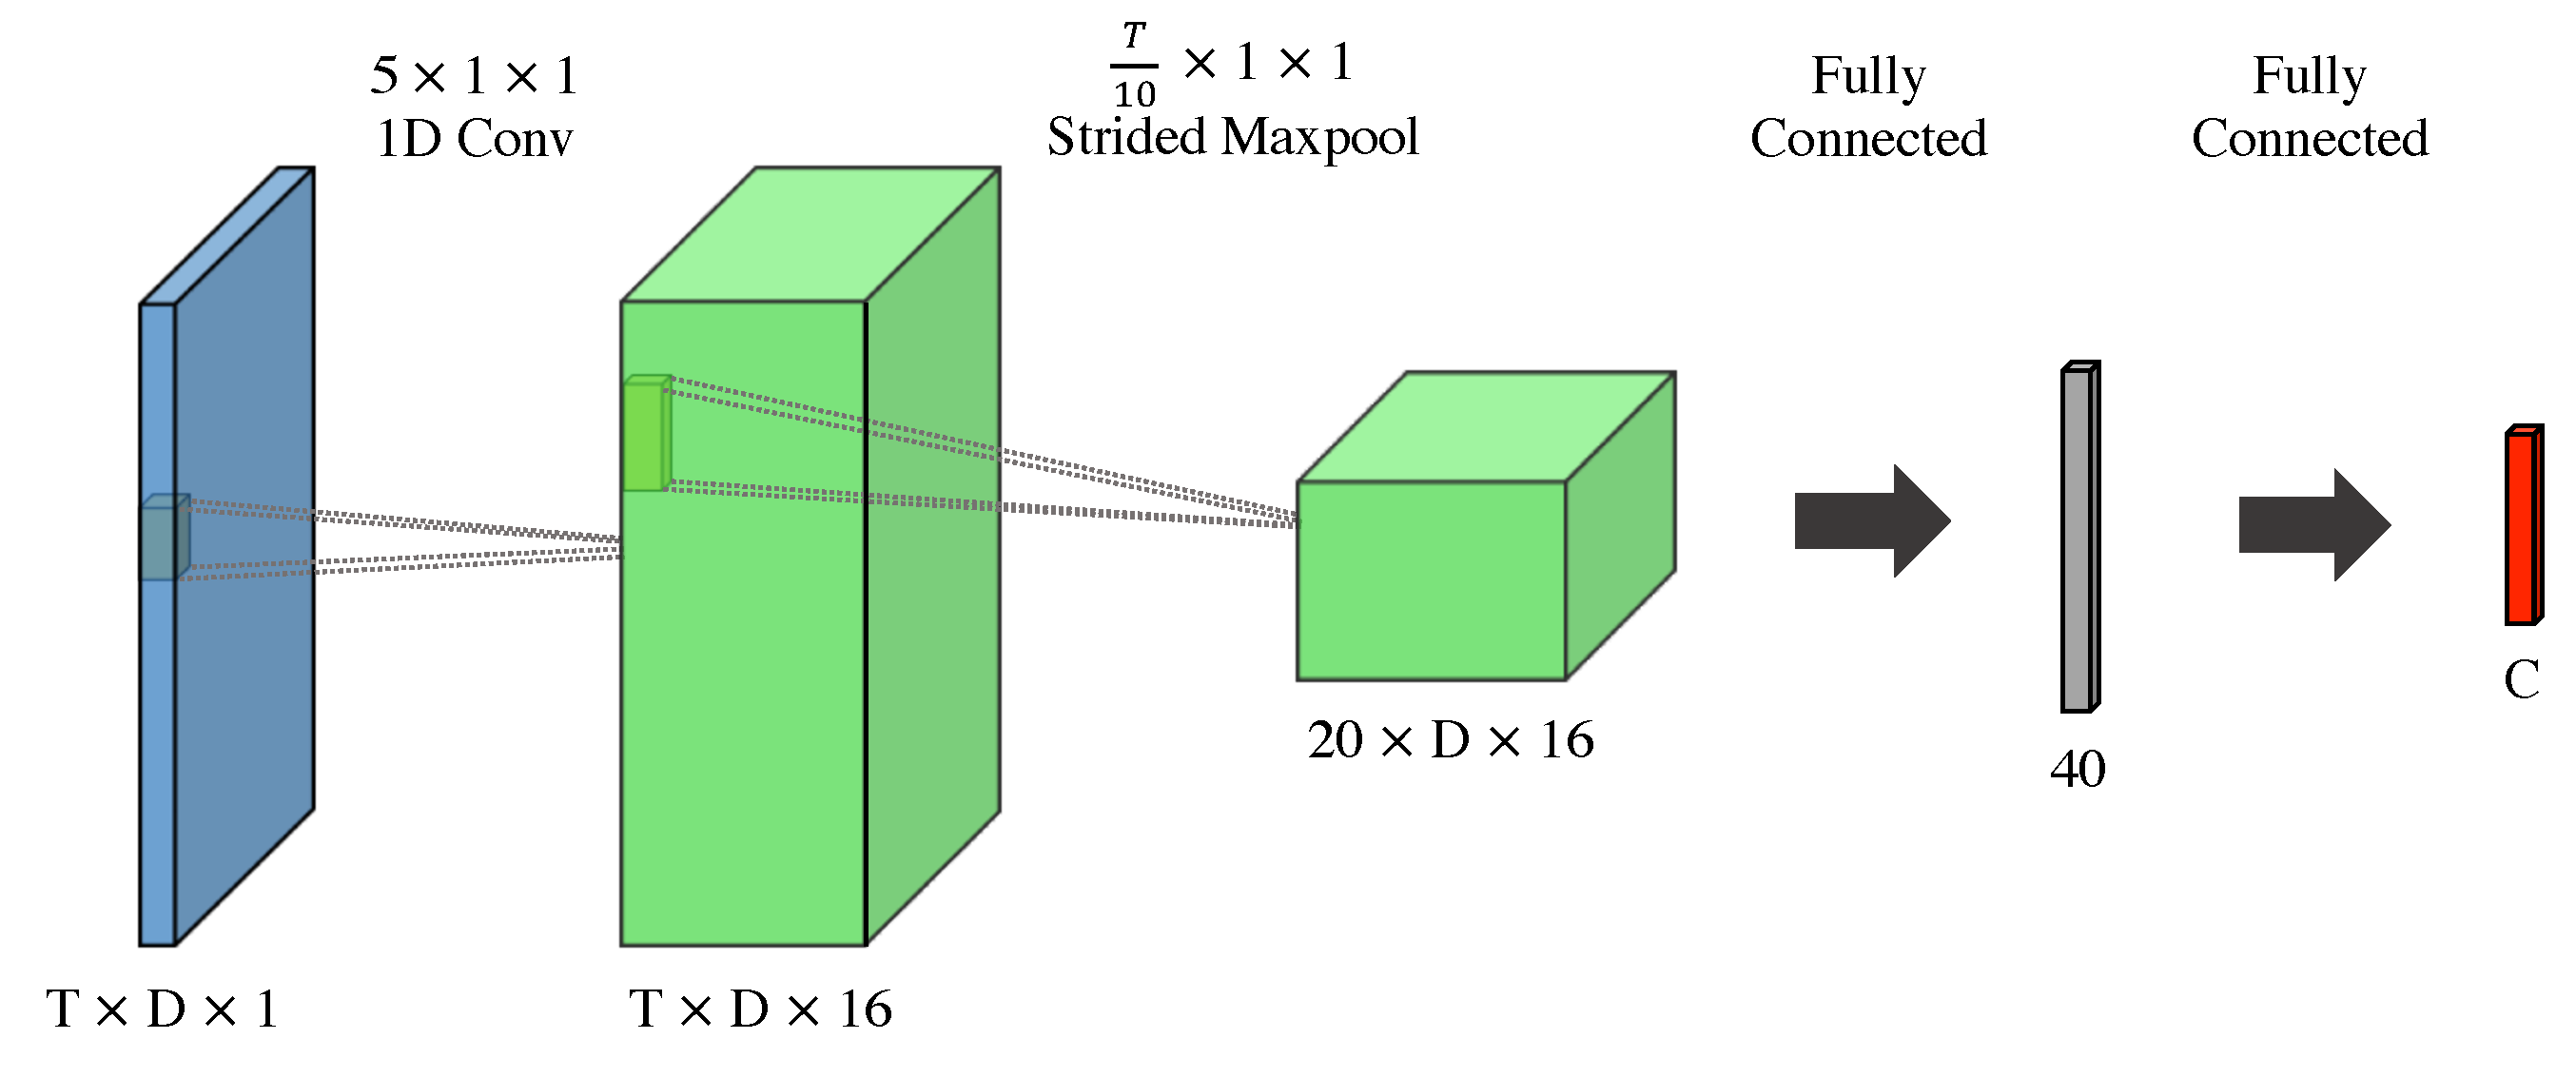
\includegraphics[width=\linewidth]{arch}
% 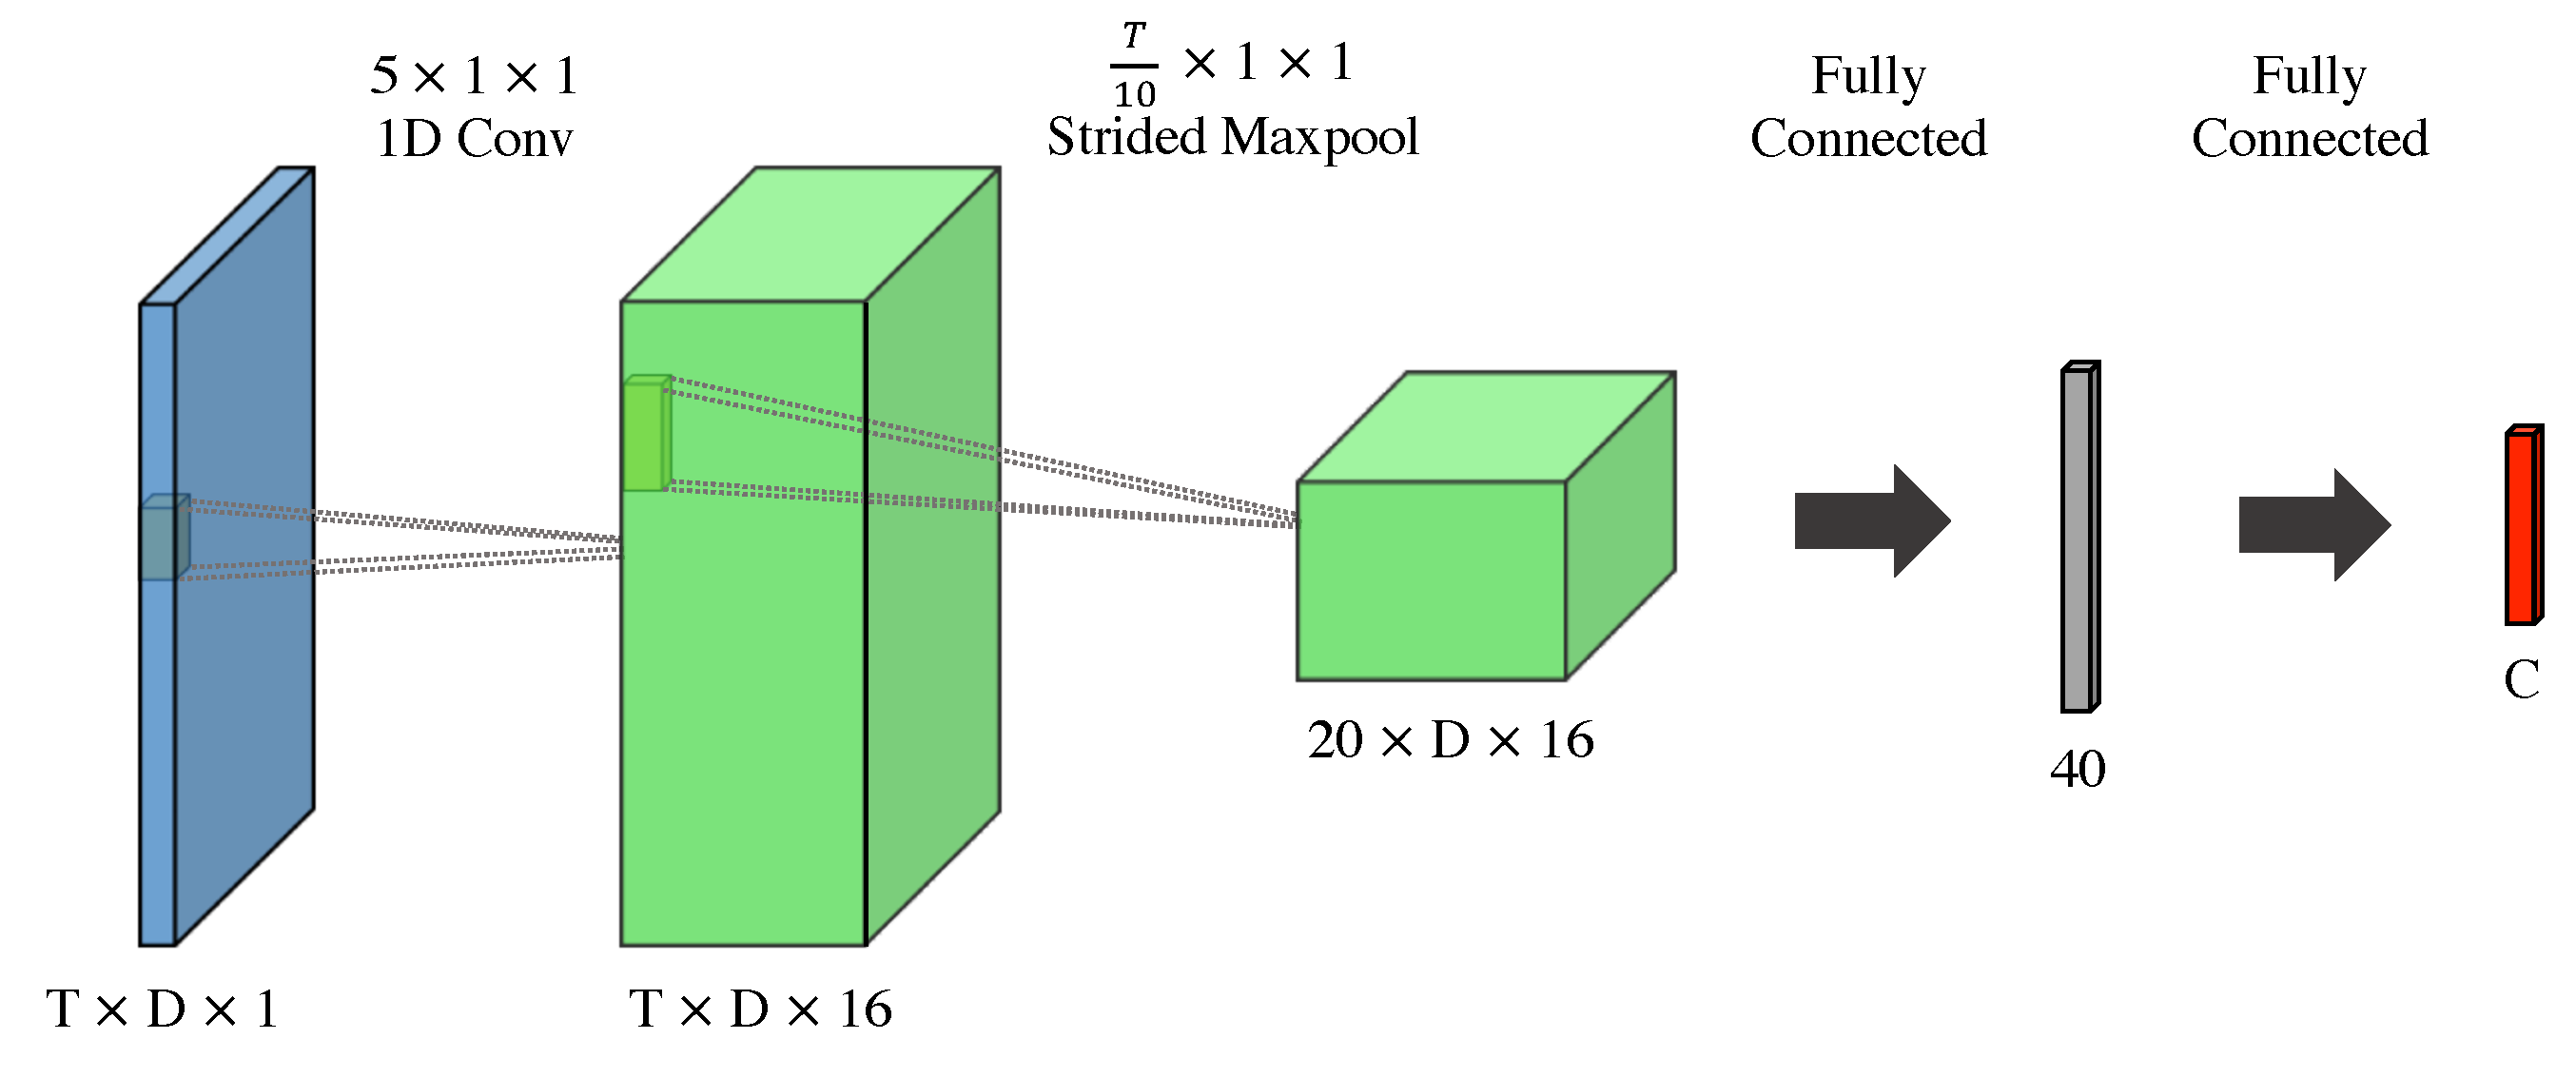
\includegraphics[width=.9\textwidth]{arch}
% % \vspace*{-2mm}
% \label{fig:arch}
% \caption{Architecture of the proposed model. TODO more explanation}
% \end{center}
% \end{figure*}



% ================================================================
\section{Method} \label{sec:method}
% ================================================================

% The network architecture is summarized in Figure~\ref{fig:arch}. The method follows the traditional format of a convolutional neural network, with one convolutional, batch normalization, and max pooling layer, followed by two fully connected layers. The chosen architecture possesses three notable considerations.  We elaborate upon these considerations below.
We learn a metric by learning to embed time series into a vector space and comparing the resulting vectors with the Euclidean distance. Our embedding function is takes the form of a convolutional neural network, shown in Figure~\ref{fig:arch}. The architecture rests on three basic layers: a convolutional layer, maxpooling layer, and a fully connected layer.

The convolutional layer is included to learn the appropriate subsequences from the input. The network employs one-dimensional filters convolved over all time steps, in contrast to traditional two-dimensional filters used with images. We opt for one-dimensional filters because time series data is characterized by infrequent sampling. Convolving over each of the variables at a given timestep has little intuitive meaning in developing an embedding when each step measurement has no coherent connection to time.  For discussion regarding the mathematical connection between a learned convolutional filter and traditional subsequence-based analysis of time series, we direct the reader to \citep{cui2016multi}.

The maxpooling layer allows the network to be resilient to translational noise in the input time series. Unlike most existing neural network architectures, the windows over which we max pool are defined as percentages of the input length, not as constants. This level of pooling allows us to heavily downsample and denoise the input signal and is fed into the final fully connected layer.

We downsample heavily after the filters are applied such that each time series is reduced to a fixed size. We do so primarily for efficiency---further discussion on parameter choice for Jiffy may be found in Section 6.

We then train the network by appending a softmax layer and using cross-entropy loss with the ADAM \citep{adam} optimizer. We experimented with more traditional metric learning loss functions, rather than a classification objective, but found that they made little or no difference while adding to the complexity of the training procedure; specific loss functions tested include several variations of Siamese networks \citep{siameseOrig,siameseRecurrent} and the triplet loss \citep{tripletMetric}. % The unsupervised network swaps the classification loss function and softmax layer for the reconstruction loss of an autoencoder. The unsupervised model is trained on a squared reconstruction loss objective function.


% We optimize our model using ADAM \citep{adam} During training time, we batch normalize after the convolutional layer.

% \vspace{8mm}

% ------------------------------------------------
\subsection{Complexity analysis}
% ------------------------------------------------

For ease of comparison to more traditional distance measures, such as DTW, we present an analysis of Jiffy's complexity.

Let $T$ be the length of the $D$-variable time series being embedded, let $F$ be the number of length $K$ filters used in the convolutional layer, and Let $L$ be the size of the final embedding.
The time to apply the convolution and ReLU operations is $\Theta(TDFK)$. Following the convolutional layer, the maxpooling and downsampling require $\Theta(T^2DF)$ time if implemented naively, but $\Theta(TDF)$ if an intelligent sliding max function is used, such as that of \citep{lemireMax}. Finally, the fully connected layer, which constitutes the embedding, requires $\Theta(TDFL)$ time.

The total time to generate the embedding is therefore $\Theta(TDF(K + L))$. Given the embeddings, computing the distance between two time series requires $\Theta(L)$ time. Note that $T$ no longer appears in either expression thanks to the max pooling.

With $F = 16$, $K = 5$, $L = 40$, this computation is dominated by the fully connected layer. Consequently, when $L \ll T$ and embeddings can be generated ahead of time, this enables a significant speedup compared to operating on the original data. Such a situation would arise, e.g., when performing a similarity search between a new query and a fixed or slow-changing database \citep{bolt}. When both embeddings must be computed on-the-fly, our method is likely to be slower than DTW and other traditional approaches. % faster than RNN-based embeddings, but % When $T < DF(K + L) = 720$,

\begin{figure*}[h]
\begin{center}
% 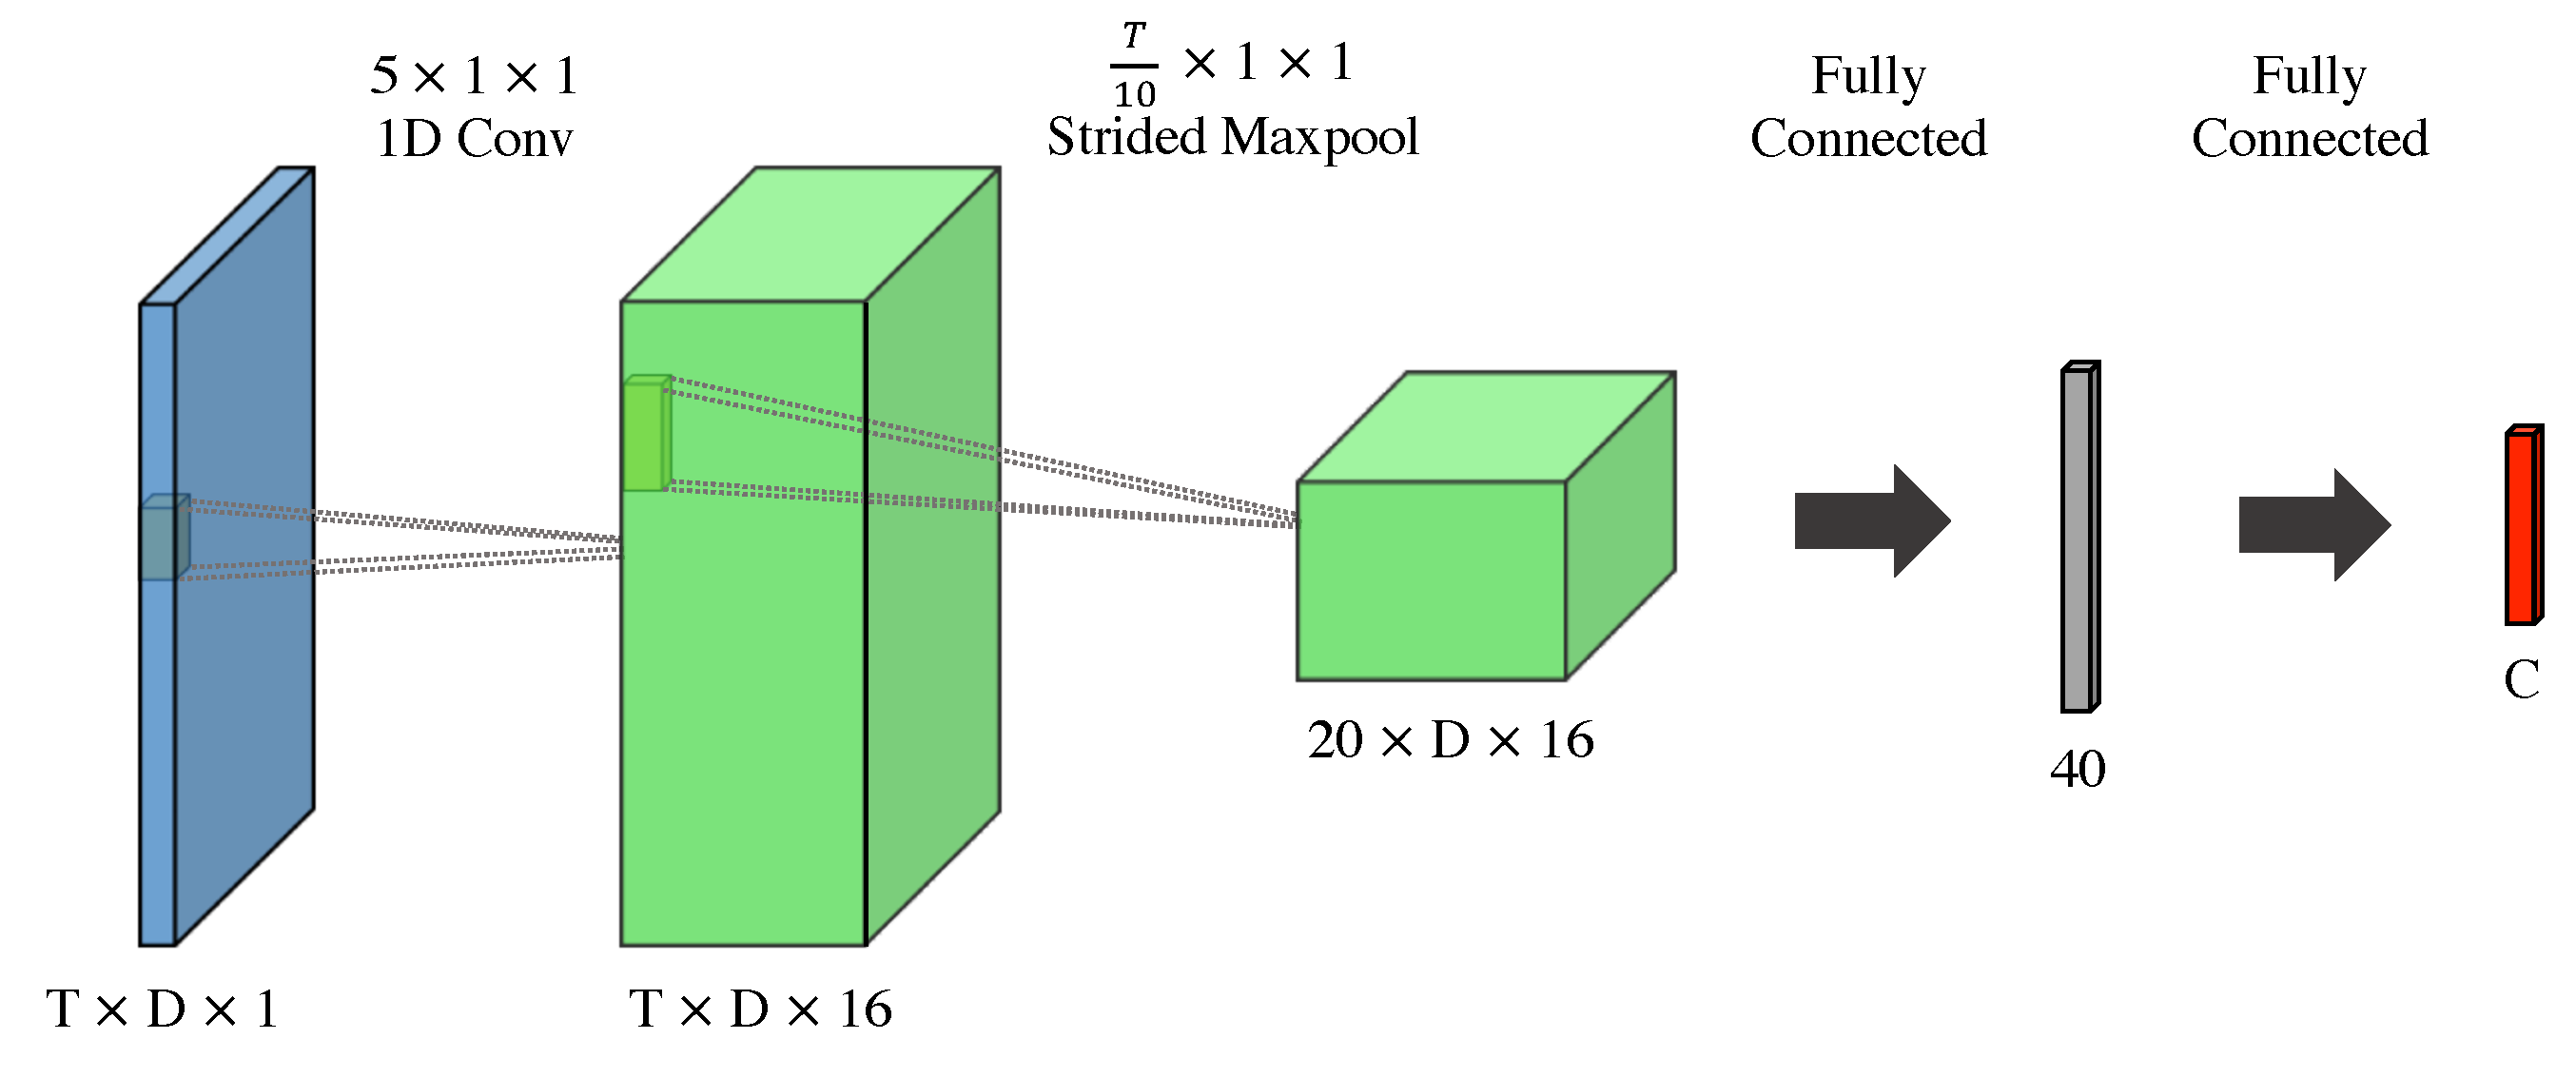
\includegraphics[width=\linewidth]{arch}
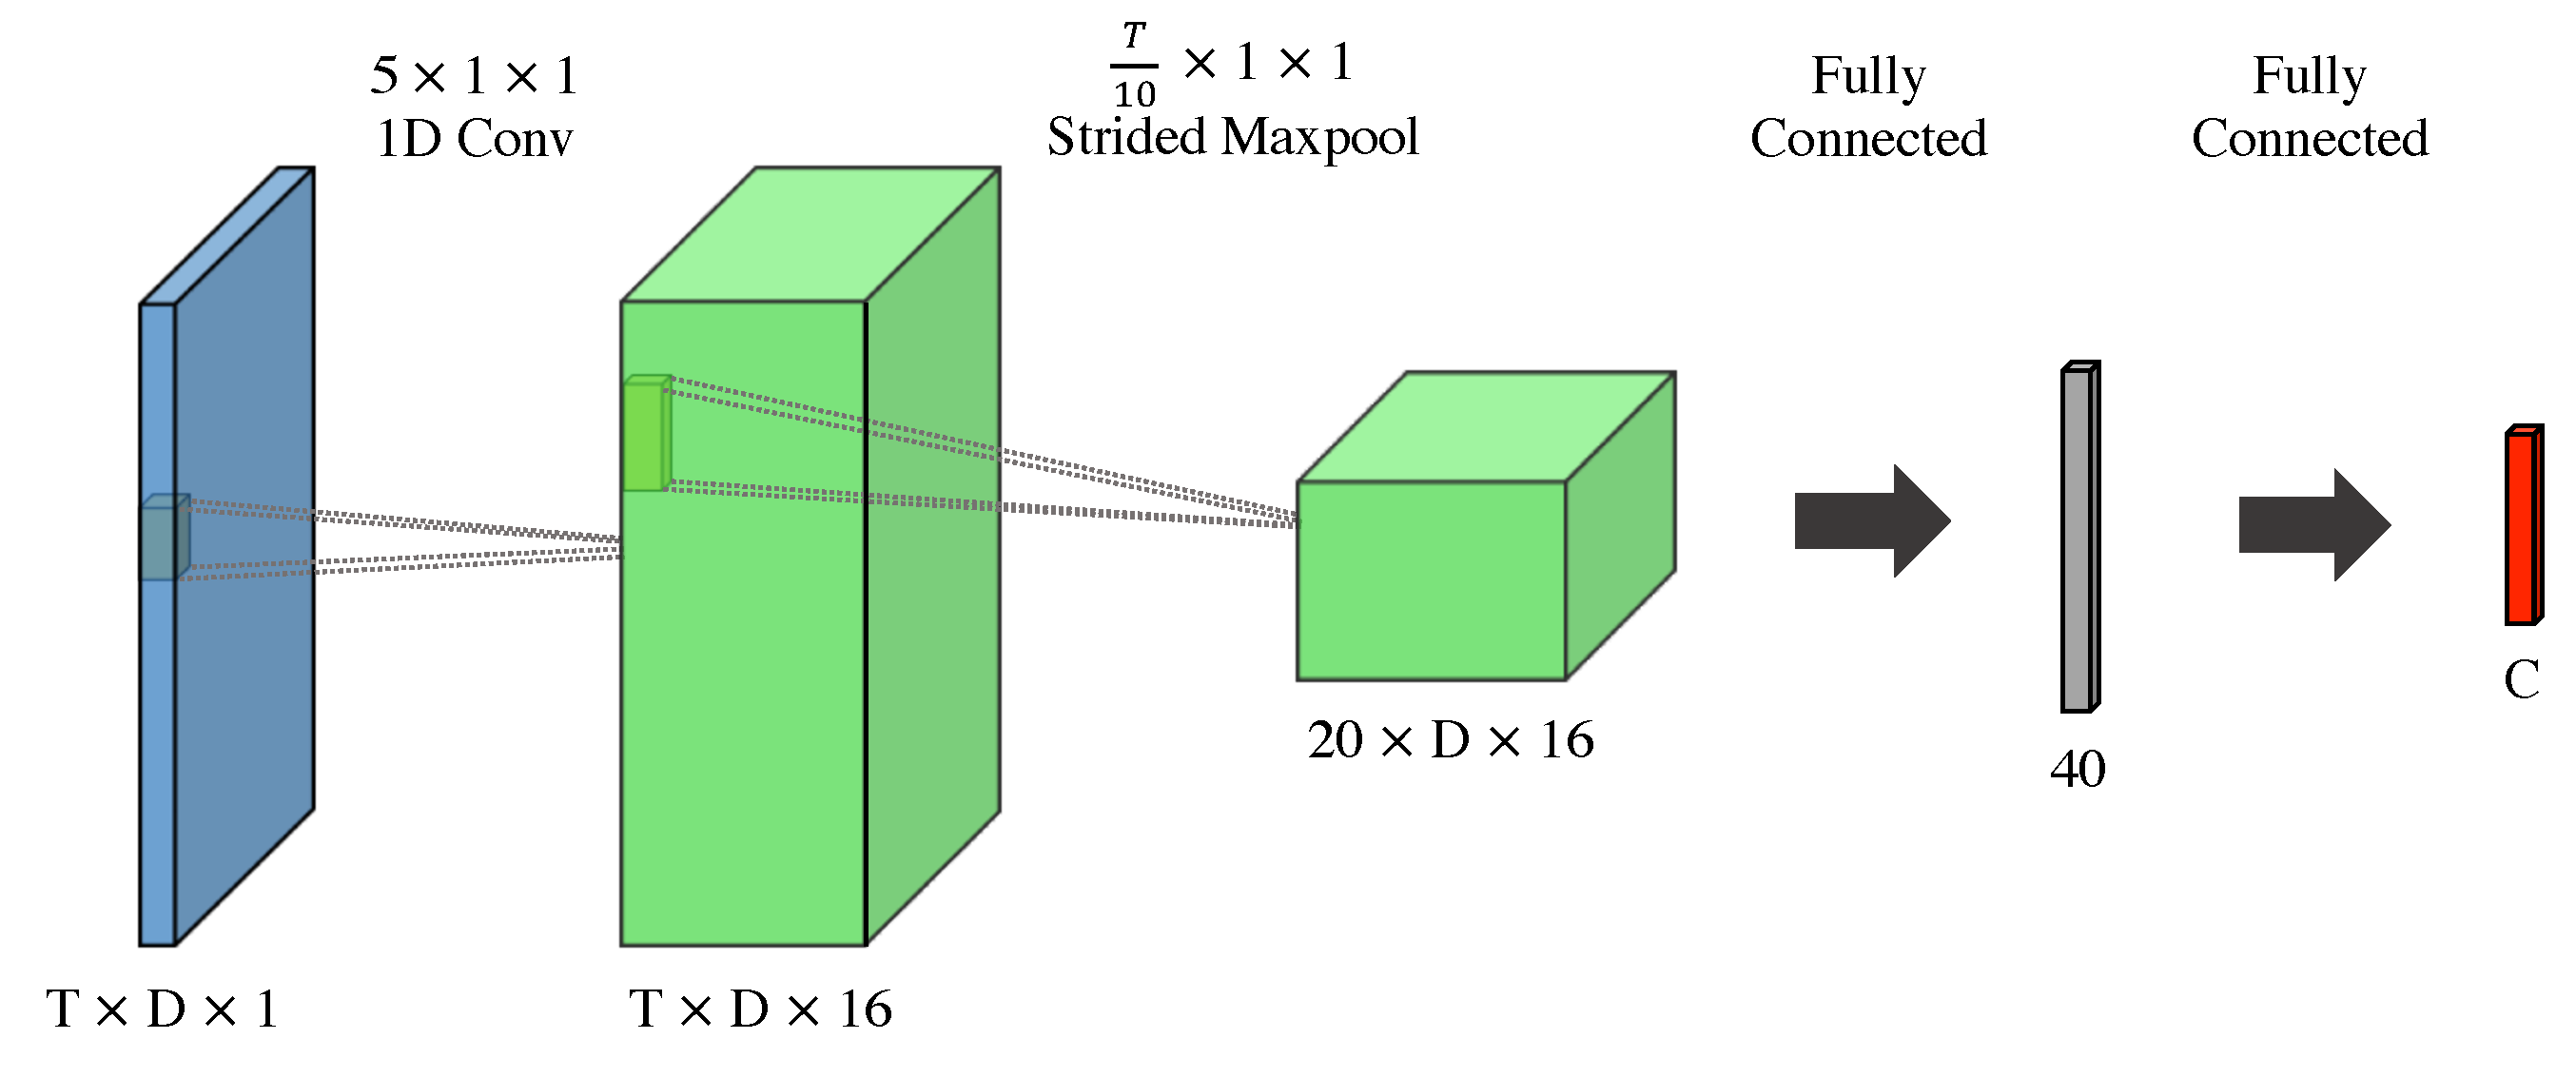
\includegraphics[width=.9\textwidth]{arch}
% \vspace*{-2mm}
\caption{Architecture of the proposed model. A single convolutional layer extracts local features from the input, which a strided maxpool layer reduces to a fixed-size vector. A fully connected layer with ReLU activation carries out further, nonlinear dimensionality reduction to yield the embedding. A softmax layer is added at training time.}
\label{fig:arch}
\end{center}
\end{figure*}
%\vspace{8m}

% \subsubsection{Bag-of-Patterns}

% Several recent representation approaches describe a time series as a set of counts detailing how many times each ``pattern'' from some fixed set takes place within it. Common patterns used include being the preimage of particular SAX words \citep{saxVSM}, or containing particular frequency content \citep{boss, weasel}.

% Our method can be seen as a continuous, trainable, relaxation of this model. First, observe that each convolutional neuron with ReLU activation can be cast as a detector for a particular pattern; when the pattern is not present, the neuron's output is 0; when it is present, the neuron's output is a continuous, rather than binary, representation of how ``present'' it is. This neuron cannot necessarily represent the exact patterns used by other methods, but if they are based on frequency content, it .

% -Suppose that each filter describes the presence of one pattern. Then if each neuron in the first fully connected layer listens to one feature map with weights tied at 1, it's just counting the number of times that pattern happens; first FC layer is then a histogram. Also note that this requires having no max pooling...


% -The first paper

% \subsubsection{Frequency-domain binning}

% Frequency-domain binning vs convolutional layers

% like shapelet stuff, but with MLP on shapelet repr, not decision tree or SVM

% // People don't seem to realize this and it's bothering me. I need to write this.



% -if one removes our fully connected layers (and adds in some additional machinery for differentiating with respect to filter length), one effectively recovers the shapelet learning algorithm of \citep{learningShapelets}. Moreover, if one further requires the shapelets to be drawn from the finite set of length $M$ subsequences observed in the data, one recovers the objective of most previous shapelet learning work.

% This can equivalently be rewritten as:
% \begin{align}
% 	\min_n \norm{\x^n - \s}^2 &= \min_n \norm{\x^n}^2 + \norm{\s}^2 - 2 \s \cdot \x^n \\
%     &= \norm{s}^2 - \frac{1}{2}\max_n \s \cdot \x^n - \norm{\x^n}^2
% %     &= b + a \max_n \s \cdot \x^n - \norm{\x^n}^2
% %     &= b + a \max_n x \ast s - \norm{\x^n}^2
% \end{align}

% \begin{align}
% 	\delta(\x, \s) \triangleq \min_n \sum_{i = 1}^{M} (x_{n - 1 + i} - s_{i})^2, M-1 < n \le N
% \end{align}
% With mean normalization, we obtain the slightly more complex:
% \begin{align}
% % \begin{split}
% 	\delta(\x, \s) \triangleq \min_n \sum_{i = 1}^{M} ( (x_{n - 1 + i} - \bar{x}_n) -
%     (s_{i} - \bar{s}) ) ^2
% % \end{split}
% \end{align}
% where
% \begin{align}
% 	\bar{s} &\triangleq \frac{1}{M} \sum_{i = 1}^{M} s_i \\
%     \bar{x}_n &\triangleq \frac{1}{M} \sum_{i = n - M + 1}^{n} x_i
% \end{align}
% Letting $\omega$ to be a vector of $M$ ones, this can be rewritten as:
% \begin{align}
% 	\delta(\x, \s) \triangleq \min_n \sum_{i = 1}^{M} ( (x_{n - 1 + i} - \bar{x}_n) -
%     (s_{i} - \bar{s}) ) ^2
% \end{align}


% \begin{align}
% % \begin{split}
% 	\delta(\x, \s) \triangleq \min_n \sum_{i = 1}^{m} \bigg( \frac{(x_{n - 1 + i} - \bar{x}_n}{\sigma_{x,n}} -
%     \frac{s_{i} - \bar{s}}{\sigma_s} \bigg) ^2
% % \end{split}
% \end{align}
% where
% \begin{align}
% 	\bar{s} &\triangleq \frac{1}{m} \sum_{i = 1}^{m} s_i \\
%     \bar{x}_n &\triangleq \frac{1}{m} \sum_{i = n - m + 1}^{n} x_i \\
%     \sigma_{x,n} &\triangleq \sqrt{ \frac{1}{m} \sum_{i = n - m + 1}^{n} (x_i - \bar{x}_n)^2}
% \end{align}


% Let $\vec{x}$ be a univariate time series and let $\s$ be a length $M$ vector. Ignoring the initial $m-1$ time steps, the convolution of $\x$ and $\s$, $\x \ast \s$, can be defined as:
% \begin{align}
% 	(\x \ast \y)(n) \triangleq \sum_{i = n-m+1}^{n} x_n y_{m - i + 1}
% \end{align}
% Suppose now that instead of treating $\vec{s}$ as a filter, we treat it as a shapelet.


% Get to here:


% -Euclidean distances are just convolving, but then negating and adding some squared norms
% -With z-normed euclidean distances, we're subtracting off output from a boxcar filter, and dividing by output from a boxcar filter over square of the time series
% 	-and also constraining the filters to live on unit hypersphere in Euclidean space
% -and biggest constraint is of course that people typically only allow shapelets that
% -shapelets max pool over whole ts, but we allow max pooling over only part of it
% -and shapelets use cross-corr, not convolution, so order is reversed

% -if one removes our fully connected layers (and adds in some additional machinery for differentiating with respect to filter length), one effectively recovers the shapelet learning algorithm of \citep{learningShapelets}. Moreover, if one further requires the shapelets to be drawn from the finite set of length $M$ subsequences observed in the data, one recovers the objective of most previous shapelet learning work.
% -fully connected layers basically mean MLP instead of linear model or decision tree on top of shapelet repr


% ================================================================
\section{Experiments} \label{sec:experiments}
% ================================================================

% Most of the aforementioned metric learning approaches apply to multivariate time series, but nearly all of the hand-crafted distance measures and representations are designed exclusively for univariate time series.

% Most could be generalized to multivariate time series in some fashion, but it is far from obvious how best to do so. For example, the Shotgun distance is based on the minimum distance between pairs of subsequences taken from each of the two time series; should the multivariate generalization take this minimum separately for each variable and sum them? Or take the minimum of these minima (or max, or median)? It could also define the subsequences to include all variables at once, or subsets of variables that are correlated, etc. In short, even for a relatively simple distance measure, the generalization to multiple variables is non-trivial.

% Because of both this and a desire to be consistent with previous time series metric learning works, we omit comparisons to univariate approaches when operating on multivariate data.

Before describing our experiments, we first note that, to ensure easy reproduction and extension of our work, all of our code is freely available.\footnote{http://smarturl.it/jiffy} All of the datasets used are public, and we provide code to clean and operate on them.

We evaluate Jiffy-produced embeddings through the task of 1-nearest-neighbor classification, which assesses the extent to which time series sharing the same label tend to be nearby in the embedded space. We choose this task because it is the most widely used benchmark for time series distance and similarity measures \citep{tsBakeoff2008,bakeoff2016}. % we would like the ``closest'' training point to a testing point in the embedded space to have the same label. % Our second set of experiments tests Jiffy in the absence of labels. In the unlabeled scenario, the ideal clustering would recreate the true labels of the data.

% We validate the classification accuracy and clustering purity of our model with six multivariate datasets sourced from a diverse range of domains. 

% ------------------------------------------------
\subsection{Datasets}
% ------------------------------------------------

To enable direct comparison to existing methods, we benchmark Jiffy using datasets employed by \citet{mddtw}. These datasets are taken from various domains and exhibit high variability in the numbers of classes, examples, and variables. We briefly describe each dataset below, and summarize statistics about each in Table~\ref{tbl:dsets}. % Due to the absence of public implementations in certain cases, we restrict our evaluation to datasets with publicly available results.

\vspace{6mm}
\begin{table*}[h]
  \centering
  \caption{Summary of Multivariate Time Series Datasets.}
  \label{tbl:dsets}
\begin{tabular}{l|c|c|c|c}
Dataset & \# Variables & \# Classes & Length & \# Time Series  \\
\hline
% EDIT: dont use the tiny datasets
% JapaneseVowels          & 12  	& 9  & 7-29 	& 640 	\\
% PenDigits            	& 2    	& 10 & 8 		& 10992 \\
Libras                	& 2    	& 15 & 45 		& 360 	\\
AUSLAN                  & 22    & 25 & 47-95 	& 675  	\\
CharacterTrajectories	& 3    	& 20 & 109-205 	& 2858 	\\ 
ArabicDigits 			& 13 	& 10 & 4 - 93 	& 8800	\\
ECG 					& 2    	& 2  & 39 - 152 & 200	\\
Wafer 					& 6    	& 2  & 104 - 198 & 1194	\\
% RobotEF - LP1 			& 6    	& 4  & 15 		& 88	\\
% RobotEF - LP2 			& 6    	& 5  & 15 		& 47	\\
% RobotEF - LP3 			& 6    	& 4  & 15 		& 47	\\
% RobotEF - LP4 			& 6    	& 3  & 15 		& 117	\\
% RobotEF - LP5 			& 6    	& 5  & 15 		& 164	\\
\end{tabular}
\label{tab:2}
% \vspace{4mm}
\end{table*}

\begin{itemize}
\item \textbf{ECG}: Electrical recordings of normal and abnormal heartbeats, as measured by two electrodes on the patients' chests.
\item \textbf{Wafer}: Sensor data collected during the manufacture of semiconductor microelectronics, where the time series are labeled as normal or abnormal.
\item \textbf{AUSLAN}: Hand and finger positions during the performance of various signs in Australian Sign Language, measured via instrumented gloves.
\item \textbf{Trajectories}: Recordings of pen (x,y) position and force application as different English characters are written with a pen. 
\item \textbf{Libras}: Hand and arm positions during the performance of various signs in Brazilian Sign Language, extracted from videos.
\item \textbf{ArabicDigits}: Audio signals produced by utterances of Arabic digits, represented by Mel-Frequency Cepstral Coefficients.
\end{itemize}

% We also use 10 datasets from the UCR Time Series Archive to demonstrate the stability of our supervised model across parameter choice.

% % ------------------------------------------------
% \subsection{Supervised Learning}
% % ------------------------------------------------
% We compared our method to a number of existing methods for the task of 1-nearest neighbor classification. We chose this task because it is widely used to benchmark time series distance measures \citep{tsBakeoff2008,bakeoff2016,mddtw}. Below, we briefly describe each method % briefly. before interpreting our results. % On subsequent experiments related to architectural considerations, we chose 10 UCR datasets to test all algorithms over. 

% ================================
% \subsubsection{Comparison Approaches}
\subsection{Comparison Approaches}
% ================================
We compare to recent approaches to time series metric learning, as well as popular means of generalizing DTW to the multivariate case: % We restrict our evaluation to approaches with published results on the tested datasets, source code provided by the authors, or sufficient simplicity that we could confidently reimplement them.

\begin{enumerate}
\item \textbf{MDDTW} \citep{mddtw} - MDDTW compares time series using a combination of DTW and the Mahalanobis distance. It learns the precision matrix for the latter using a triplet loss.
\item \textbf{Siamese RNN} \citep{siameseRecurrent} - The Siamese RNN feeds each time series through a recurrent neural network and uses the hidden unit activations as the embedding. It trains by feeding pairs of time series through two copies of the network and computing errors based on their inner products in the embedded space.
\item \textbf{Siamese CNN} The Siamese CNN is similar to the Siamese RNN, but uses convolutional, rather than recurrent, neural networks. This approach has proven successful across several computer vision tasks \citep{siameseOrig,taigman2014deepface}. 
\item \textbf{DTW-I}, \textbf{DTW-D} - As pointed out by \citet{nontrivial}, there are two straightforward ways to generalize DTW to multivariate time series. The first is to treat the time series as $D$ independent sequences of scalars (DTW-I). In this case, one computes the DTW distance for each sequence separately, then sums the results. The second option is to treat the time series as one sequence of vectors (DTW-D). In this case, one runs DTW a single time, with elementwise distances equal to the squared Euclidean distances between the $D$-dimensional elements.
 \item \textbf{Zero Padding} - One means of obtaining a fixed-size vector representation of a multivariate time series is to zero-pad such that all time series are the same length, and then treat the ``flattened'' representation as a vector.
 \item \textbf{Upsampling} - Like Zero Padding, but upsamples to the length of the longest time series rather than appending zeros. This approach is known to be effective for univariate time series \citep{everythingWrongDTW}.
\end{enumerate}

% ================================
% \subsubsection{Results}
\subsection{Accuracy}
% ================================
 % Below, we briefly describe each method % briefly. before interpreting our results. % On subsequent experiments related to architectural considerations, we chose 10 UCR datasets to test all algorithms over. 

As shown in Table~\ref{tbl:results}, we match or exceed the performance of all comparison methods on each of the six datasets. Although it is not possible to claim statistical significance in the absence of more datasets (see \cite{cdDiagrams}), the average rank of our method compared to others is higher than its closest competitors at 1.16. The closest second, DTW-I, has an average rank of 3.33 over these six datasets.
 
Not only does Jiffy attain higher classification accuracies than competing methods, but the method also remains consistent in its performance across datasets. This can most easily be seen through the standard deviation in classification accuracies across datasets for each method. Jiffy's standard deviation in accuracy (0.026) is approximately a third of DTWI's (0.071). The closest method in terms of variance is MDDTW with a standard deviation of 0.042 , which exhibits a much lower rank than our method. This consistency suggests that Jiffy generalizes well across domains, and would likely remain effective on other datasets not tested here.

\vspace{5mm}
\begin{table*}[h] % each row is an algorithm/model; each col is a dataset
  \centering
  \caption{1NN Classification Accuracy. The proposed method equals or exceeds the accuracies of all others on every dataset.}
\label{tbl:results} % label needs to go after caption
\begin{tabular*}{\textwidth}{l|c|ccccccc}
Dataset                & Jiffy      & MDDTW & DTW-D  & DTW-I     & \makecell{Siamese \\ CNN} & \makecell{Siamese \\ RNN} & \makecell{Zero \\ Pad} & Upsample \\
\hline
ArabicDigits           & \b{0.974}  & 0.969 &  0.963 & \b{0.974} &    0.851   & 0.375      &    0.967   &   0.898   \\
AUSLAN                 & \b{1.000}  & 0.959 &  0.900 & \b{1.000} & \b{1.000}  & \b{1.000}  &\b{1.000}   & \b{1.000} \\
ECG                    & \b{0.925}  & 0.865 &  0.825 &    0.810  &    0.756   & 0.659      &    0.820   &   0.820   \\
Libras                 & \b{1.000}  & 0.908 &  0.905 &    0.979  &    0.280   & 0.320      &    0.534   &   0.534   \\
Trajectories           & \b{0.979}  & 0.961 &  0.956 &    0.972  &    0.933   & 0.816      &    0.936   &   0.948   \\
Wafer                  & \b{0.992}  & 0.988 &  0.984 &    0.861  &    0.968   & 0.954      &    0.945   &   0.936   \\
\hhline{=|=|=======}
 Mean Rank              & \b{1.67}   & 3.67  & 4.67   & 3.33      &  6.0       & 6.5        &  4.17      & 4.5     \\
\end{tabular*}
\vspace{4mm}
\end{table*}

% % ------------------------------------------------
% \subsection{Unsupervised Learning}
% % ------------------------------------------------

% More often than not, multivariate time series exist unlabeled, with no known set of classes. Even in the labeled case, there may be \textit{too many} labels. This is especially prevalent in medicine, where the notion of similarity between patients is important to such tasks as cohort selection, diagnosis, and treatment but but the process of labeling is heavily noisy.  We examine the performance of our model on the clustering task to demonstrate its value in unsupervised settings.

% % ================================
% \subsubsection{Comparison Approaches}
% % ================================

% We compare our model to four recent approaches to unsupervised time series clustering. The algorithms we compare to operate on the basis of unsupervised representation learning. Additionally, we include both the zero-padded representation of the multivariate time series and the up-sampled representation as a baseline comparison. Each competing algorithm's methodology is described briefly below: 

% \begin{enumerate}
% \item \textbf{LDPS} \citep{ldps} - LDPS uses a single-layer CNN to embed time series such that the Euclidean distance between time series $T_a$ and $T_b$ in the transformed space approximates the DTW distance between $T_a$ and $T_b$ in the original space. 
% \item \textbf{SPIRAL} \citep{spiral} - SPIRAL is similar to LDPS in that it learns a time series feature space in which DTW similarity is preserved. Notably, SPIRAL's approach is based on matrix factorization.
% \item \textbf{Zero Padding} - One means of obtaining a fixed-size vector representation of a multivariate time series is to zero-pad such that all time series are the same length, and then treat the ``flattened'' representation as a vector.
% \item \textbf{Upsampling} - Like Zero Padding, but upsamples to the length of the longest time series rather than appending zeros. This approach is known to be effective for univariate time series \citep{everythingWrongDTW}.
% % \item \textbf{U-Shape} \citep{ushapelets} - U-Shape creates and iteratively refines clusters by repeatedly dividing the dataset using entropy-reducing shapelets. 
% \end{enumerate}

% % ================================
% \subsubsection{Results}
% % ================================

% We evaluate our method using the Rand Index, a common cluster evaluation metric. As Table \ref{tbl:clusteringResults} demonstrates, Jiffy achieves higher clustering purities than all competing methods, save for the upsampling baseline. We may draw the following conclusions from our results:

% \begin{itemize}
% 	\item Given the competitive performance of the upsampling baseline, it is important to note that the objective of our work is to build a generalizable metric for multiple machine learning tasks. The upsampling baseline performs very poorly in the classification task, implying that Euclidean distance in the original, untransformed space does not adequately describe similarity between multivariate time series.
%     \item Both SPIRAL and LDPS, our primary comparison methods, demonstrate a lower rank than the two baselines we have chosen as well. This speaks to their potential specialization to univariate time series.
%     \item The dimensionality across each of the representations learned by each of these methods varies greatly. For example, the upsampling baseline uses 615 features for each multivariate time series instance in the CharacterTrajectories dataset. On the other hand, Jiffy uses only 2 and produces a superior clustering.
% \end{itemize}

% \begin{table}[h]
%   \centering
% \begin{tabular}{l|c|cccc}
% Dataset                 &  Jiffy    & LDPS      & SPIRAL & Zero-Padding & Upsampling \\
% \hline
% ArabicDigits            &    0.849  &    0.826  & 0.870  &    0.887     & \b{0.928} \\
% AUSLAN                  & \b{0.990} & \b{0.990} & 0.868  &    0.982     &    0.982  \\
% CharacterTrajectories   & \b{0.965} &    0.939  & 0.886  & \b{0.965}    &    0.959  \\
% ECG                     &    0.586  &    0.550  & 0.505  &    0.581     & \b{0.627} \\
% Libras                  &    0.883  &    0.870  & 0.881  & \b{0.885}     &\b{0.885} \\
% Wafer                   & \b{0.746} &    0.554  & 0.448  &    0.500     &    0.596  \\
% \hhline{=|=|====}
% \b{Mean Rank}		& 	2.0	&	3.67		& 4.5	&	2.5		&	\b{1.83}
% \end{tabular}

% \vspace{4mm}
% \caption{Rand Indices of k-means clustering using various learned representations. Despite having no labels and reducing the dimensionality by orders of magnitude relative to the zero-padded or upsampled data, Jiffy yields no loss in performance. Jiffy also equals or outperforms existing unsupervised representation learning methods. } %It is important to note that the upsampled and zero-padded representation of Libras are the same because its a fixed length dataset.}
% \label{tbl:clusteringResults}
% \end{table}






% ================================================================
\section{Hyperparameter Effects} \label{sec:network}
% ================================================================

%A natural question when considering the performance of a neural network is whether, or to what extent, the hyperparameters must be modified to achieve good performance on a new dataset. Jiffy's consistent performance across the above datasets using fixed hyperparameters suggests that little modification is required. To assess this further, however, we measured the changes in Jiffy's performance on additional datasets while varying two parameters that were especially likely to affect performance in early experiments---the embedding size and the amount of maxpooling.

A natural question when considering the performance of a neural network is whether, or to what extent, the hyperparameters must be modified to achieve good performance on a new dataset. In this section, we explore the robustness of our approach with respect to the values of the two key parameters: embedding size and pooling percentage. We do this by learning metrics for a variety of parameter values for ten data sets from the UCR Time Series Archive \citep{ucrArchive}, and evaluating how classification accuracy varies.

%Jiffy's consistent performance across the above datasets using fixed hyperparameters suggests that little modification of th is required, but to assess this further, we run

%Because they are widely used, we chose 10 datasets at random from the UCR time series archive \cite{ucrArchive}.

% In the interest of exploring the stability of our model's performance with respect to parameter choice without tuning our network to the test datasets, we rigorously test parameter choices against a suite of 10 datasets from the UCR Time Series Archive. We explore two parameters in particular: embedding size and pooling percentage.

% ================================
\subsection{Embedding Size}
% ================================

%The plot on the left of Figure \ref{fig:params} 
Figure \ref{fig:params}.\textit{left} shows that even a few dozen neurons are sufficient to achieve peak accuracy. As a result, an embedding layer of 40 neurons is sufficient and leads to an architecture that is compact enough to run on a personal laptop.

% It is apparent that after a certain point additional neurons have little to no effect in the utility of the embedding for classification.

\begin{figure}[h]
\begin{center}
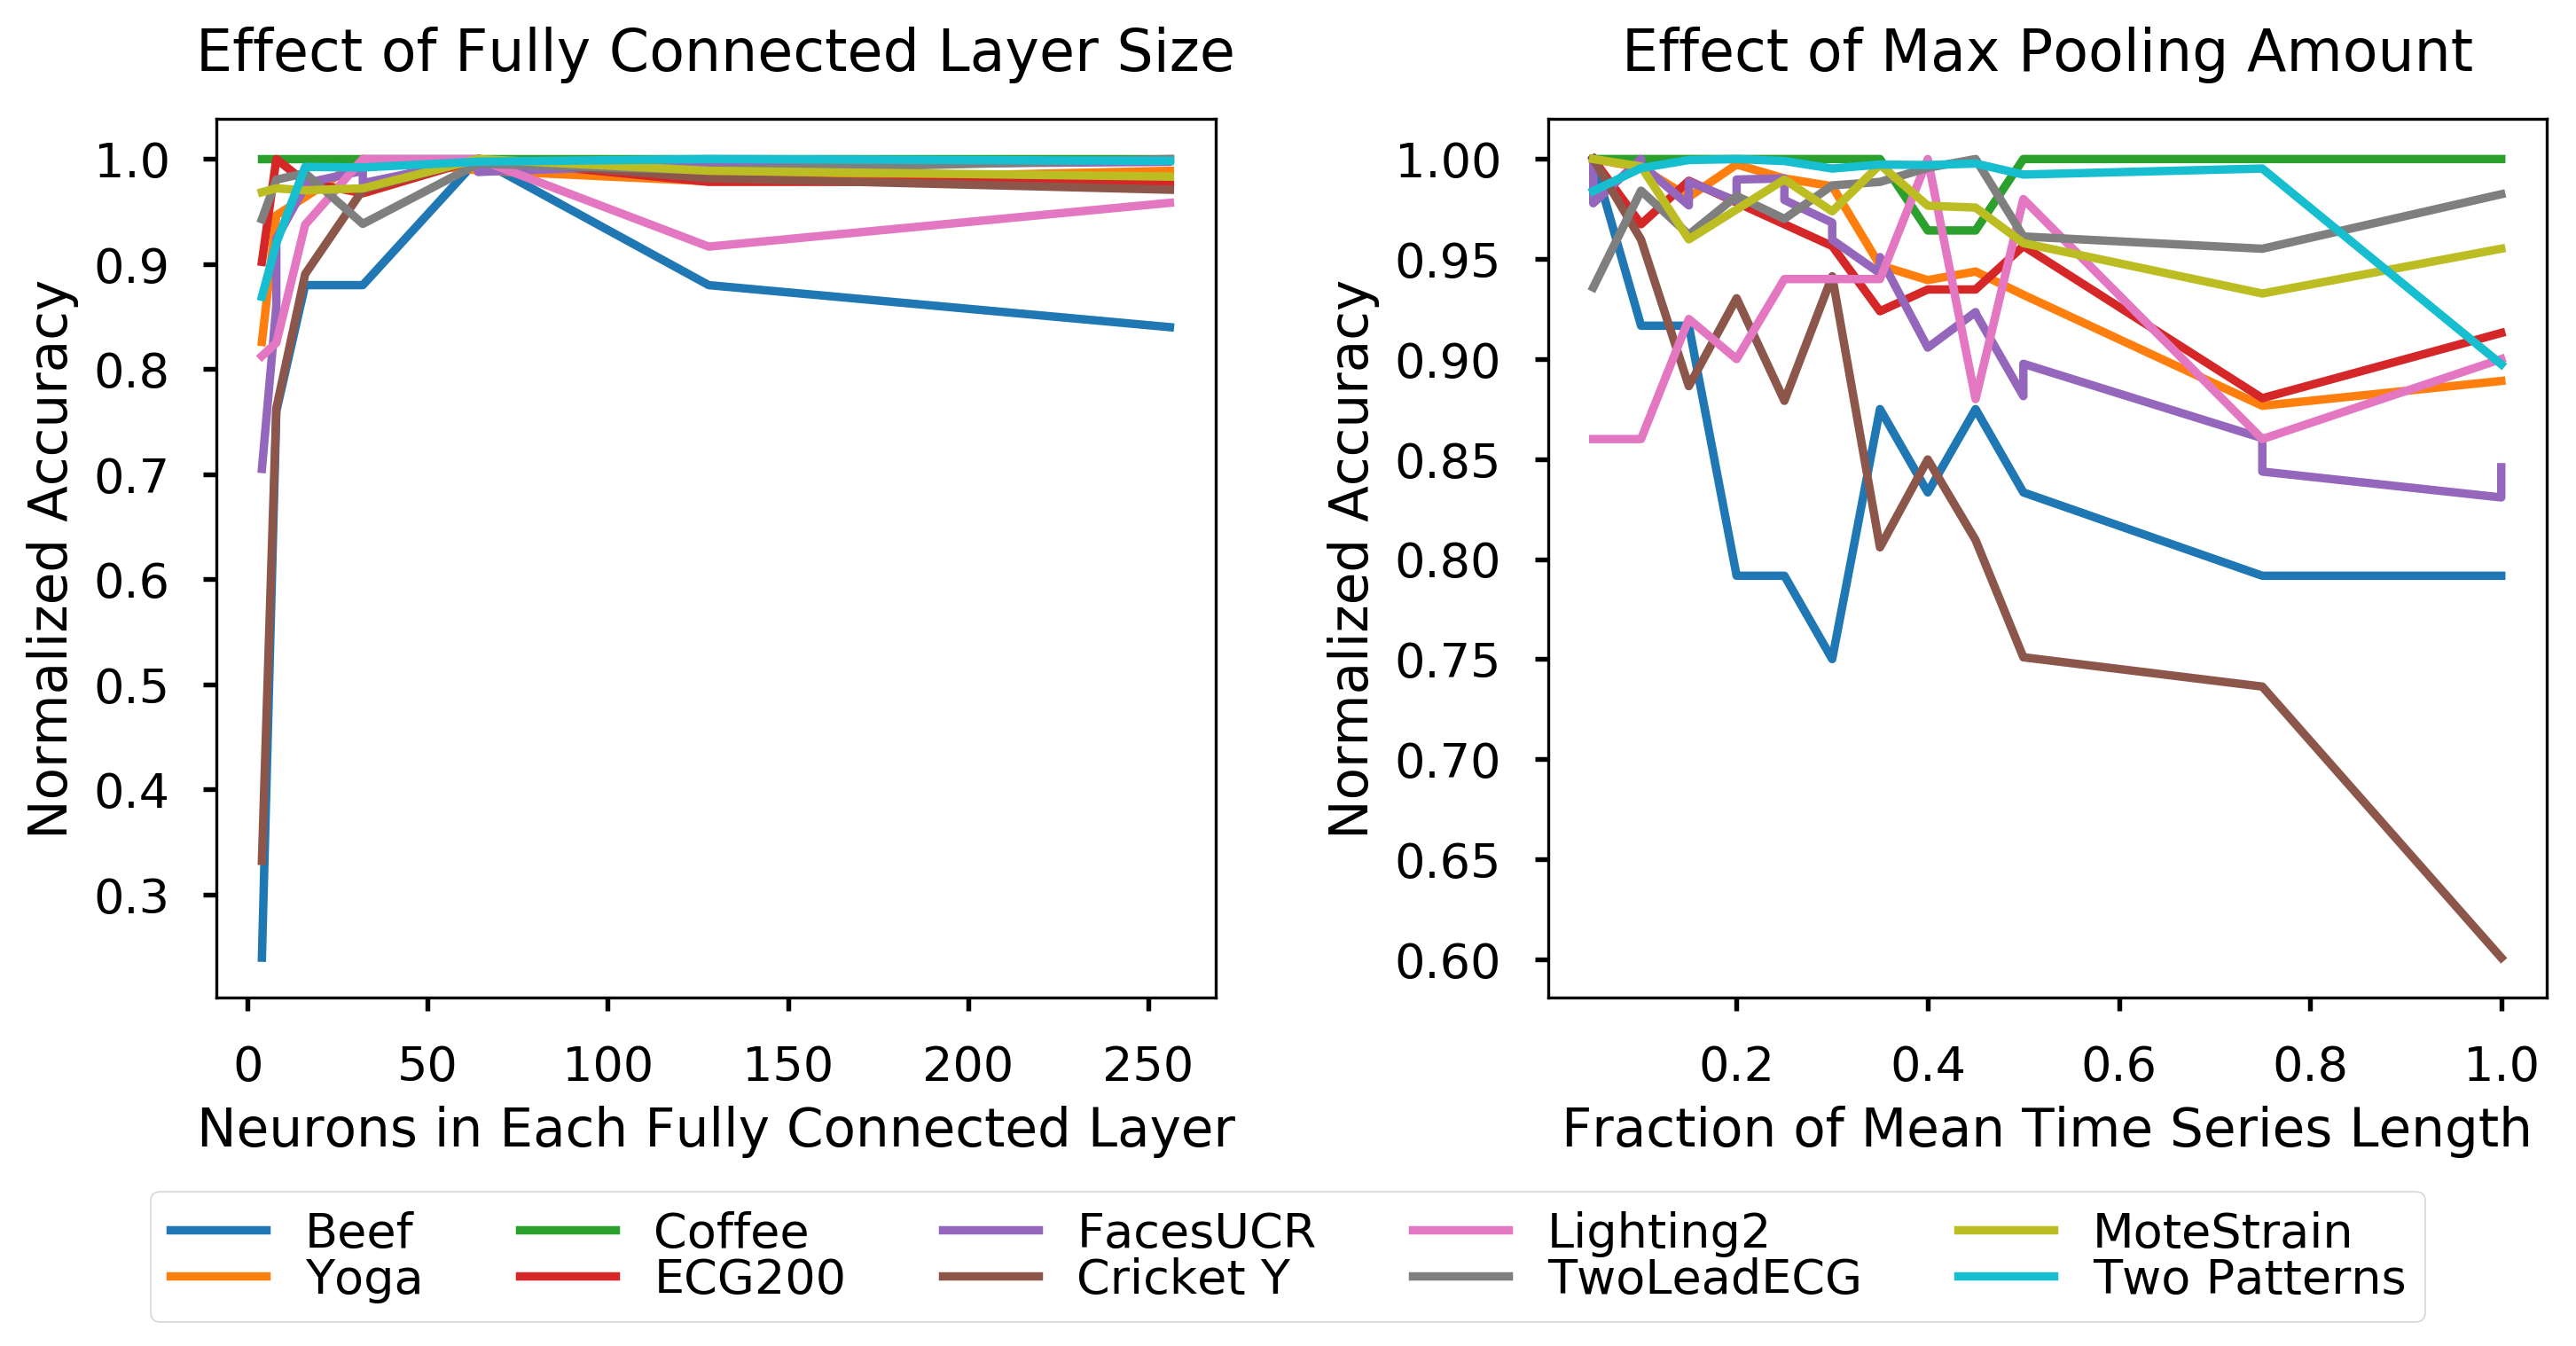
\includegraphics[width=\linewidth]{param_effects}
\vspace*{-5mm}
\caption{Effect of fully connected layer size and degree of max pooling on model accuracy using held-out datasets. Even small fully connected layers and large amounts of max pooling---up to half of the length of the time series in some cases---have little or no effect on accuracy. For ease of visualization, each dataset's accuracies are scaled such that the largest value is 1.0.}
\label{fig:params}
\end{center}
\end{figure}

% ================================
\subsection{Pooling percentage}
% ================================
% This method is especially common in shapelet-based classification procedures in which a candidate shapelet is convolved across the entire time series in an attempt to find the closest distance between the given shapelet and a subsequence of the time series.

The typical assumption in machine learning literature is that max pooling windows in convolutional architectures should be small to limit information loss. In contrast, time series algorithms often max pool globally across each example (e.g. \citep{learningShapelets}). Contrary to the implicit assumptions of both, we find that the level of pooling that results in the highest classification often falls in the 10-25\% range, as shown by Figure \ref{fig:params}.\textit{right} % the plot on the right side of Figure \ref{fig:params}.

% \subsection{Unsupervised Learning}

% % ================================
% \subsubsection{Embedding Size}
% % ================================
% In line with our observation in the supervised setting, we see (Figure~\ref{fig:params_unsupervised}) that embedding size has little to no effect on the quality of the autoencoder architecture's produced clustering. This aligns with our understanding of time series data; each of these datasets is inherently low dimensional and the negligible clustering purity increase as the embedding size grows reflects that.

% % ================================
% \subsubsection{Pooling Percentage}
% % ================================
% We observe a similar phenomenon to the supervised setting in that we are able to pool broadly at no cost to the resulting cluster purity (Figure ~\ref{fig:params_unsupervised}). This behavior contradicts previous approaches to pooling over time series; other methods use globally averaged filters or fixed width windows. 

% \begin{figure}[h]
% \begin{center}
% 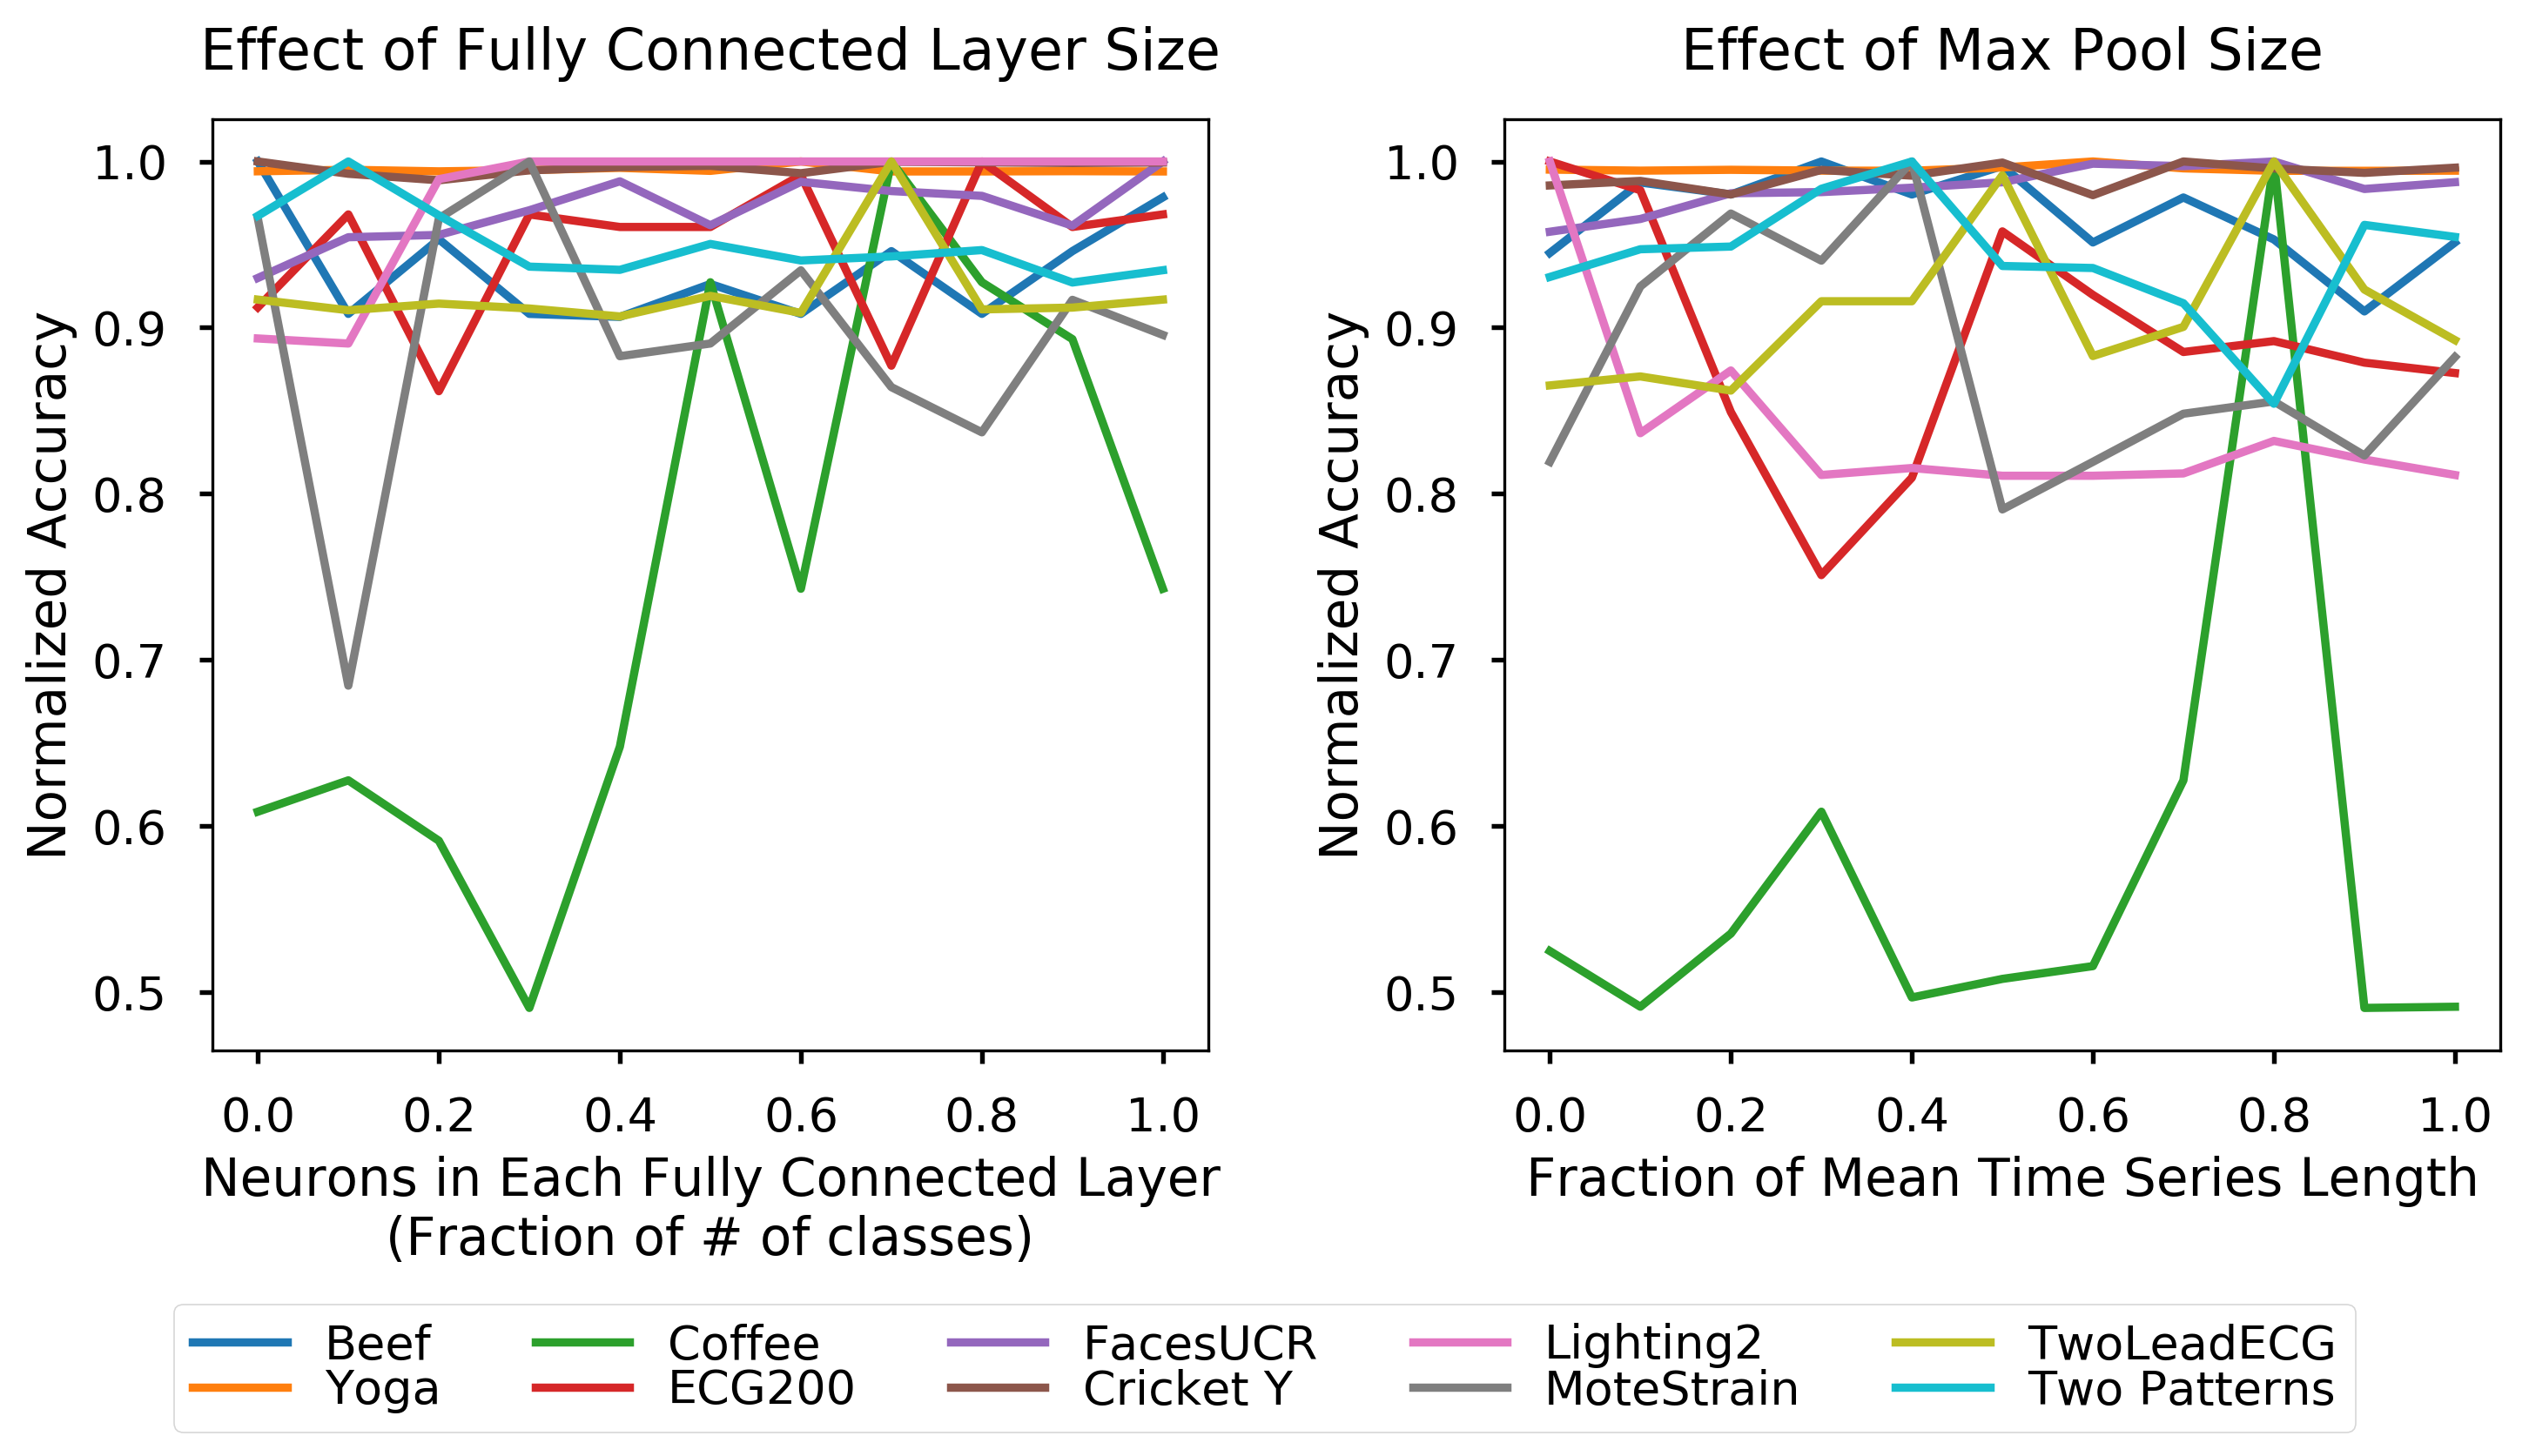
\includegraphics[width=\linewidth]{param_effects_unsupervised}
% \vspace*{-5mm}
% \caption{Effect of fully connected layer size and degree of max pooling on model accuracy using held-out datasets. Even small fully connected layers and large amounts of max pooling---up to half of the length of the time series in some cases---have little or no effect on accuracy. For ease of visualization, each dataset's accuracies are scaled such that the largest value is 1.0.}
% \label{fig:params_unsupervised}
% \end{center}
% \end{figure}





% ================================================================
\vspace{-1mm}
\section{Conclusion} \label{sec:conclusion}
% ================================================================

We present Jiffy, a simple and efficient metric learning approach to measuring multivariate time series similarity. We show that our method learns a metric that leads to consistent and accurate classification across a diverse range of multivariate time series. Jiffy's resilience to hyperparameter choices and consistent performance across domains provide strong evidence for its utility on a wide range of time series datasets.

Future work includes the extension of this approach to multi-label classification and unsupervised learning. There is also potential to further increase Jiffy's speed by replacing the fully connected layer with a structured \citep{structuredMats} or binarized \citep{xnornet} matrix. % during both training and inference time.

% \bibliographystyle{aaai}
% \bibliographystyle{abbrev}
% \bibliographystyle{iclr2018_conference}
% \bibliography{doc}
\bibliographystyle{ACM-Reference-Format}
\bibliography{main}

\end{document}
